\documentclass[11pt]{article}
% Built with Tectonic (XeTeX). In VS Code, saving rebuilds the PDF; see README.md.
\usepackage[a4paper,margin=2.5cm]{geometry}
\usepackage{amsmath}
\usepackage{unicode-math}
\setmainfont{Helvetica}
\setsansfont{Helvetica}
\setmonofont{Menlo}[Scale=MatchLowercase]
\setmathfont{STIX Two Math}
% Helvetica for Greek and digits in inline maths, so they match the text.
\setmathfont{Helvetica}[range={up/{Latin,latin,Greek,greek,num}, it/{Latin,latin,Greek,greek}}]
% Word pasted maths symbols as plain text; the text font lacks them.
\usepackage{newunicodechar}
\newunicodechar{∇}{\ensuremath{\nabla}}
\newunicodechar{∝}{\ensuremath{\propto}}
\newunicodechar{∥}{\ensuremath{\parallel}}
\newunicodechar{≈}{\ensuremath{\approx}}
\newunicodechar{≥}{\ensuremath{\geq}}
\newunicodechar{⊥}{\ensuremath{\perp}}
\newunicodechar{𝐵}{\ensuremath{\mathit{B}}}
\newunicodechar{𝑆}{\ensuremath{\mathit{S}}}
\newunicodechar{𝑒}{\ensuremath{\mathit{e}}}
\newunicodechar{𝑖}{\ensuremath{\mathit{i}}}
\newunicodechar{𝑙}{\ensuremath{\mathit{l}}}
\newunicodechar{𝑚}{\ensuremath{\mathit{m}}}
\newunicodechar{𝑛}{\ensuremath{\mathit{n}}}
\newunicodechar{𝑜}{\ensuremath{\mathit{o}}}
\newunicodechar{𝑣}{\ensuremath{\mathit{v}}}
\newunicodechar{𝑥}{\ensuremath{\mathit{x}}}
\newunicodechar{µ}{\ifmmode\mupmu\else\char"B5\fi}
\newunicodechar{𝜎}{\ensuremath{\sigma}}
\usepackage{graphicx}
\usepackage{longtable,booktabs,array,calc}
\usepackage{etoolbox}
\AtBeginEnvironment{longtable}{\footnotesize\setstretch{1.1}}
\AtBeginEnvironment{tabular}{\setstretch{1.1}}
\setlength{\LTpre}{8pt}\setlength{\LTpost}{4pt}
\usepackage{xcolor}
\definecolor{linkblue}{HTML}{1F4E9A}
\usepackage[authoryear,round,sort]{natbib}
\setlength{\bibsep}{2pt}
\setlength{\bibhang}{1.5em}
\usepackage{tikz}
\usetikzlibrary{arrows.meta,positioning,fit,backgrounds,calc}
\usepackage[colorlinks=true,linkcolor=black,citecolor=linkblue,urlcolor=linkblue]{hyperref}
\usepackage{authblk}
\usepackage{orcidlink}
\newcommand{\doilink}[1]{\href{https://doi.org/#1}{\nolinkurl{#1}}}
% Review markers, both removed before submission.
% \tocheck: value from the Word draft, not yet confirmed against the code.
% \revised: value or sentence changed to match the corrected code/re-solve.
% To hide both, change their bodies to {#1}.
\definecolor{revisedorange}{HTML}{C05600}
\newcommand{\tocheck}[1]{#1}
\newcommand{\revised}[1]{#1}
\usepackage{setspace}
\onehalfspacing
\usepackage[running]{lineno}
\linenumbers
\renewcommand\linenumberfont{\normalfont\scriptsize}
\usepackage[labelfont=bf,labelsep=period,font=small,singlelinecheck=false]{caption}
\usepackage{fancyhdr}
\pagestyle{fancy}
\fancyhf{}
\fancyfoot[C]{\small\thepage}
\renewcommand{\headrulewidth}{0pt}
\fancypagestyle{plain}{\fancyhf{}\fancyfoot[C]{\small\thepage}}
\usepackage{titlesec}
\titleformat{\section}{\normalfont\large\bfseries}{\thesection.}{0.5em}{}
\titleformat{\subsection}{\normalfont\normalsize\bfseries}{\thesubsection}{0.5em}{}
\titlespacing*{\section}{0pt}{16pt}{4pt}
\titlespacing*{\subsection}{0pt}{10pt}{2pt}
\graphicspath{{figures/}}
% Never break a word across lines. Extra stretch lets TeX spread a line
% instead of pushing a long word into the margin.
\hyphenpenalty=10000
\exhyphenpenalty=10000
\emergencystretch=3em
\tolerance=2000
\setlength{\parskip}{0pt}
\setlength{\parindent}{1.5em}
\renewcommand\Authfont{\normalsize}
\renewcommand\Affilfont{\small}
\setlength{\affilsep}{8pt}
\makeatletter
\renewcommand{\maketitle}{%
  \thispagestyle{plain}%
  \begingroup\setstretch{1.15}\centering
  {\Large\bfseries\@title\par}\vspace{14pt}%
  {\@author\par}%
  \endgroup\vspace{12pt}}
\makeatother
\renewenvironment{abstract}
  {\section*{Abstract}\noindent\ignorespaces}
  {\par\vspace{4pt}}

\title{iNOB: an open software package for whole-body bioelectromagnetic forward modelling for experimental design}

\author[1,*,\textdagger]{Oliver Case\,\orcidlink{0009-0007-4499-0682}}
\author[3,\textdagger]{Maike Schmidt\,\orcidlink{0009-0001-6307-0095}}
\author[3]{Harry Cook\,\orcidlink{0000-0002-4794-4119}}
\author[4]{Stephanie Mellor\,\orcidlink{0000-0001-8164-645X}}
\author[5,6]{George C. O'Neill\,\orcidlink{0000-0002-0035-3768}}
\author[3]{Nicholas A. Alexander\,\orcidlink{0000-0001-5161-684X}}
\author[1]{Pier D. Lambiase\,\orcidlink{0000-0002-9055-9267}}
\author[2]{Sarah N. Garfinkel\,\orcidlink{0000-0002-5961-1012}}
\author[3,\textdaggerdbl]{Gareth R. Barnes\,\orcidlink{0000-0002-5396-7712}}

\affil[1]{UCL Centre for Neurocardiology, Institute of Cardiovascular Science, University College London, London, United Kingdom}
\affil[2]{Institute of Cognitive Neuroscience, University College London, London, United Kingdom}
\affil[3]{Department of Imaging Neuroscience, UCL Queen Square Institute of Neurology, University College London, London, United Kingdom}
\affil[4]{Translational Neuromodeling Unit (TNU), Institute for Biomedical Engineering, University of Zurich \& ETH Zurich, Z\"urich, Switzerland}
\affil[5]{Department of Neuroscience, Physiology and Pharmacology, University College London, London, United Kingdom}
\affil[6]{FieldLine Medical, Louisville, CO, United States}
\date{}

\begin{document}
\maketitle
\begin{center}
{\small\setstretch{1.15}
\textsuperscript{*}Corresponding author: Oliver Case, \href{mailto:oliver.case.25@ucl.ac.uk}{oliver.case.25@ucl.ac.uk}\par
\textsuperscript{\textdagger}These authors contributed equally and are joint first authors.\par
\textsuperscript{\textdaggerdbl}Senior author.\par}
\end{center}

\begin{abstract}
Bioelectromagnetic source imaging has largely focused on the brain, yet
the peripheral and autonomic nervous systems generate signals that, in
principle, can also be recorded non-invasively. When planning to record
from a region of interest, the required number of sensors, their
positions and the number of trials should ideally be estimated, based on
an appropriate forward model and sensor type. To support this task we
present iNOB (imaging Neuroscience Outside the Brain), an open-source
software package for forward modelling and sensor planning based on a
whole-body template. The user selects a target structure and source
configuration (location, number and strength of dipoles), chooses which
anatomical meshes to include and their conductivities, and generates a
magnetometer array (for example, optically pumped magnetometers) and/or
a surface-electrode array. From this information, a pipeline is run to
create triangulated atlas meshes, from which a multi-tissue tetrahedral
finite-element model is used to calculate magnetic and electric
leadfields in absolute units. Finite-element solutions are benchmarked
against analytic spherical-conductor (Sarvas) solutions to show where
simpler models are and are not adequate. Using our tool, we present
experimental designs to image the spinal cord, vagus nerve, and a set of
neck muscles, highlighting the advantages to be gained from our
target-specific approach. iNOB is intended for experimental design
rather than inverse solutions: it estimates what a given array could
detect before data are collected. The complete package, unit tests and
figure scripts are released under the MIT licence.
\end{abstract}

\noindent\textbf{Keywords:} \emph{magnetography; optically pumped magnetometers;
vagus nerve; spinal cord; finite element method; electroneurography.}

\section{Introduction}\label{introduction}

Magnetocardiography (MCG) and electrocardiography of the heart,
magnetospinography (MSG) of the spinal cord and magnetogastrography
(MGG) of the stomach each recover physiologically meaningful signal from
outside the skull.

Recording these signals from outside the head is relatively well
established, depending on the region in question. However, to perform
source imaging, and so infer where recorded activity originates, a model
of the anatomy is required to calculate how signals propagate from
source to sensor. The same model tells us what current sensor technology
can and cannot measure, so that the pipelines and methodologies that
already exist for the brain can be extended to the whole body. This is
where `forward modelling' comes in.

In the context of bioelectric and biomagnetic source imaging, a forward
model is a causal description of how the measured data arise; here it
answers a narrow question: if a known source of electrical activity sits
at a known place inside the body, what magnetic field, or what electric
potential, appears at a sensor on the skin? Answering it requires a
description of how current spreads through the intervening tissue,
because bone, fat, muscle and blood conduct very differently, and
because that spread determines the amplitude and spatial profile of
electromagnetic signals at the skin surface. Because neighbouring
tissues interact in shaping this spread, the volume conductor has to be
modelled as a whole rather than tissue by tissue. The resulting map from
every candidate source to every sensor is called the leadfield, and it
is the object that every source reconstruction method ultimately depends
on. Forward modelling \citep{227} has been used since the very early
days of magnetoencephalography (MEG) and electroencephalography (EEG)
\citep{195, 196, 226, 228}. Although the earliest biomagnetic
measurements were in fact of the heart (Baule \& McFee, 1963),
source-level forward modelling outside the head has since received
comparatively little attention (but see van Oosterom \& Oostendorp,
2004, for the heart, and O'Neill et al., 2025, and
Schmidt et al., 2026, for the spinal cord).

Existing forward modelling platforms and solvers are, with some specific
exceptions, optimised specifically for the brain. This largely reflects
where the field's interest has been: most source
localisation work targets the brain, so tissue surfaces, source spaces
and sensor layouts are all set up to expect head anatomy. For MEG, the
head's approximately spherical geometry also permits
analytic simplifications that are not available elsewhere in the body;
for EEG, which is far more sensitive to the conductivities of skull and
scalp, realistic-geometry models are the norm. Beyond the spherical
approximation, two more general methods instead represent the true
geometry of the brain, skull, scalp and other head tissues: the boundary
element method (BEM) and the finite element method (FEM)
\citep{235, 236, 237, 238}.

BEM represents only the surfaces separating one tissue from the next,
and treats everything between two surfaces as a single uniform
homogeneous material that conducts equally well in every direction
(isotropic). FEM instead divides the whole volume into many small
elements, typically tetrahedra, so that conductivity can vary from place
to place and, within a single element, can differ by direction. This
directional dependence is called anisotropy.

The assumptions of BEM are reasonable for the brain, skull and scalp,
but are harder to justify in tissues such as skeletal muscle, myocardium
and peripheral nerves, whose fibre architecture makes conductivity
strongly direction dependent and whose anatomy does not reduce to a
small set of nested closed surfaces.

Extension of these methods to geometries and tissue types beyond the
head has begun, most notably for the spinal cord \citep{233, 175, 234},
but remains in its early stages and is more specific to use cases.
Elsewhere in the body, detailed forward modelling has been applied to
specific peripheral structures: ASCENT \citep{202}, for instance, models
intrafascicular vagus nerve anatomy in fine detail, but it is built for
invasive simulation studies and does not produce non-invasive,
electromagnetic source imaging-style forward solutions.

The gap, then, is not a shortage of good tools but the absence of a
single pipeline that lets an investigator specify an arbitrary
anatomical region and modality and obtain a comparable answer.

MEG and EEG refer, by construction, to electrophysiological recordings
from the brain. Because iNOB is concerned with structures outside the
brain, we use the target-neutral terms \emph{magnetography} (MG) and
\emph{electrography} (EG) throughout, reserving MEG and EEG for the
brain and using target-specific forms
(magnetospinography/electrospinography, MSG/ESG, for the spinal cord;
magnetoneurography, MNG, for nerve; magnetomyography/electromyography,
MMG/EMG, for muscle) where a particular structure is meant. This follows
a convention already established in the field, where
magnetocardiography, magnetospinography and magnetomyography are named
for their targets rather than treated as variants of MEG.

We present iNOB, a generalisable FEM framework for modelling a variety
of body structures, including the spinal cord, peripheral nerve and
muscle, within one consistent pipeline, and accessible to investigators
without specialised meshing or numerical-methods expertise. It is built
to answer one question: for any structure in the body, what would a
sensor on the skin surface measure, and, for a stated noise level, how
many trials would be needed to detect it?

iNOB does not introduce a new numerical solver: the volume-conduction
problem is solved by DUNEuro \citep{242}, the anatomy is derived from
BodyParts3D \citep{241}, and the surface and volume meshing steps use
established libraries (trimesh, PyMeshFix \citep{244}, iso2mesh
\citep{245}/CGAL). What is new is the layer built on top of them,
outlined below:

(1) First, sensor arrays are generated automatically for arbitrary body
regions, so a magnetometer array (of any type, with the noise level and
stand-off from the skin set by the user; defaults approximate wearable
optically pumped magnetometers (OPMs)) or a surface-electrode array can
be placed over the neck, torso or a limb without a hand-built,
region-specific sensor definition.

(2) Second, the magnetic and electric forward solutions are computed
from the same tetrahedral model under the same conductivity assignment
and calibrated against analytic references to physical units (fT and µV
per nA·m), so MG and EG predictions for a given target are directly
comparable, rather than being expressed in the solver's
raw, dimensionally ambiguous output units.

(3) Third, a physiological layer, applied after the leadfield
calculation, maps fibre-level source assumptions to dipole moments,
dipole moments to sensor amplitudes, and sensor amplitudes to the number
of averaged trials required to detect the source at a stated noise
floor, which is the quantity an experimenter needs before committing to
a recording.

The underlying solver is validated elsewhere \citep{243}; what we
validate here are these three additions.

\section{The iNOB framework}\label{the-inob-framework}

iNOB is configuration-driven: a single YAML file is the source for the
target structure, the meshes included in the volume conductor, their
conductivities, the source space (location, spacing, number and strength
of dipoles), the sensor arrays and the noise floors, with any of these
fields overridable from the command line or GUI. From these inputs, the
package:

\begin{quote}
(i) maintains a curated atlas of watertight triangulated meshes derived
from BodyParts3D (Mitsuhashi et al., 2009);

(ii) builds a multi-tissue tetrahedral model by voxel shrink-wrapping and
CGAL meshing;

(iii) places magnetometers (single-axis or triaxial, with user-specified
noise level and stand-off from the skin) and surface-electrode arrays
automatically on the relevant body surface;

(iv) computes both the MG and EG forward models from the same base model
with DUNEuro, calibrated to absolute units; and

(v) estimates detectability (predicted signal-to-noise ratio (SNR) and
the number of averaged trials required) for a chosen source and noise
floor.
\end{quote}

The pipeline runs end to end from one command, \texttt{inob run}, with \revised{twenty-seven}
subcommands covering the individual stages, twenty-three of which can
also be called as standalone console scripts. It can equally be driven
from a browser-based graphical interface (Figure 1), a FastAPI backend
with a React/TypeScript front end, in which the user edits the
configuration, previews the meshes, presses run, and watches each stage
stream its log live over a websocket. Every stage that produces an
output file (for example, a mesh or a leadfield) validates it against a
documented on-disk schema before writing, and revalidates it on load
before the next stage consumes it; every run is seeded from a single
configurable seed for reproducibility. The package is about \revised{24,000} lines
of MIT-licensed Python, or \revised{37,000} including tests, alongside a
\revised{9,600}-line TypeScript front end, with a suite of \revised{1,072} tests run in
continuous integration on Python 3.11 and 3.12.

\begin{figure}[htbp]
\centering
% Figure 1: the iNOB pipeline, top to bottom. The model-building stages run
% down the left; sources join from the right; both meet at the forward solve.
\begin{tikzpicture}[
    font=\sffamily,
    node distance=0.62cm and 1.6cm,
    stage/.style={draw=black!75, line width=0.55pt, rounded corners=2pt, fill=white,
      text width=4.6cm, minimum height=0.95cm, align=center, inner sep=3pt,
      execute at begin node={\setlength{\parindent}{0pt}\setstretch{1}\centering\hyphenpenalty=10000\exhyphenpenalty=10000}},
    goal/.style={stage, line width=1.1pt, draw=black},
    flow/.style={-{Stealth[length=4.5pt,width=3.6pt]}, line width=0.6pt, draw=black!80},
    edge/.style={font=\ttfamily\scriptsize, text=black!60, inner sep=3pt},
  ]
  % \stage[style]{name}{number}{title}{subtitle}{placement}
  \newcommand{\stagetext}[3]{{\footnotesize\bfseries #1\,\,#2}\\[-1pt]{\scriptsize\color{black!60}#3}}

  \node[stage]                   (mod) {\stagetext{1}{Modality}{MEG, EEG or both}};
  \node[stage, below=of mod]     (ana) {\stagetext{2}{Anatomy}{tissue surfaces for the target region}};
  \node[stage, below=of ana]     (con) {\stagetext{3}{Conductivities}{one value per tissue}};
  \node[stage, below=of con]     (fem) {\stagetext{4}{FEM meshing}{multi-tissue tetrahedral volume}};
  \node[stage, below=of fem]     (sen) {\stagetext{5}{Sensor array}{OPMs and/or surface electrodes}};
  \node[stage, right=of sen]     (src) {\stagetext{6}{Sources}{dipole location, orientation, strength}};
  \node[stage, below=0.9cm of $(sen.south)!0.5!(src.south)$] (fwd)
        {\stagetext{7}{Forward solve}{DUNEuro finite-element leadfield}};
  \node[goal, below=of fwd]      (tri) {\stagetext{8}{Trials to detect}{amplitude, SNR and averages needed}};

  \draw[flow] (mod) -- node[edge, right] {meg/eeg}  (ana);
  \draw[flow] (ana) -- node[edge, right] {surfaces} (con);
  \draw[flow] (con) -- node[edge, right] {sigma}    (fem);
  \draw[flow] (fem) -- node[edge, right] {volume}   (sen);
  \draw[flow] (sen.south) |- ++(0,-0.45) -| node[edge, above, pos=0.25] {sensors} ([xshift=-6pt]fwd.north);
  \draw[flow] (src.south) |- ++(0,-0.45) -| node[edge, above, pos=0.25] {dipoles} ([xshift=6pt]fwd.north);
  \draw[flow] (fwd) -- node[edge, right] {leadfield} (tri);
\end{tikzpicture}

\caption{The iNOB pipeline. Each node is a processing stage and each
edge a data dependency, labelled with the artefact the upstream stage
writes and the downstream stage consumes: the recording modality, the
tissue surfaces of the selected anatomy, their conductivities
($\sigma$), the tetrahedral volume, the sensor or electrode array, the
source dipoles and the leadfield. The same graph drives the web
interface, where an edge is highlighted once its upstream stage has
written its outputs, source position and orientation are specified
interactively in a three-dimensional view of the selected anatomy, and
each stage streams its log as the run proceeds. The terminal stage
reports the predicted sensor-level amplitude and the number of averaged
trials required to detect the specified source at the configured noise
floor.}
\label{fig:1}
\end{figure}

\begin{longtable}[]{@{}
  >{\raggedright\arraybackslash}p{(\linewidth - 4\tabcolsep) * \real{0.2637}}
  >{\raggedright\arraybackslash}p{(\linewidth - 4\tabcolsep) * \real{0.2570}}
  >{\raggedright\arraybackslash}p{(\linewidth - 4\tabcolsep) * \real{0.4793}}@{}}
\caption{The iNOB command-line surface. Most commands are also
available as a standalone console script, given in the second column;
the two spellings dispatch to the same code.}\label{tab:1}\\
\toprule
\textbf{Command} & \textbf{Legacy binary} & \textbf{Description} \\
\midrule
\endfirsthead
\multicolumn{3}{@{}l}{\small\textbf{Table 1} (continued)}\\[3pt]
\toprule
\textbf{Command} & \textbf{Legacy binary} & \textbf{Description} \\
\midrule
\endhead
\bottomrule
\endlastfoot
\addlinespace[4pt]
\multicolumn{3}{@{}l}{\textit{Start here}} \\
\addlinespace[1pt]
\texttt{inob doctor} & -- & Check that the host machine can run the pipeline \\
\texttt{inob status} & -- & Report which stages are built and what to run next \\
\texttt{inob run} & \texttt{inob-pipeline} & Run the whole pipeline, geometry through to
leadfield \\
\addlinespace[4pt]
\multicolumn{3}{@{}l}{\textit{Build the model}} \\
\addlinespace[1pt]
\texttt{inob build-geom} & \texttt{inob-build-geom} & Surface meshes to watertight
anatomical geometry \\
\texttt{inob build-fem} & \texttt{inob-build-fem} & Geometry to multi-tissue tetrahedral
FEM mesh \\
\texttt{inob sensors} & \texttt{inob-sensors} & \revised{Magnetometer array: triaxial, single-axis, or imported} \\
\texttt{inob electrodes} & \texttt{inob-electrodes} & Place the high-density
surface-electrode array \\
\addlinespace[4pt]
\multicolumn{3}{@{}l}{\textit{Solve (requires duneuropy)}} \\
\addlinespace[1pt]
\texttt{inob forward} & \texttt{inob-forward} & Magnetography leadfield via DUNEuro \\
\texttt{inob eeg} & \texttt{inob-eeg} & Electrography leadfield via DUNEuro \\
\texttt{inob volume-field} & \texttt{inob-volume-field} & Solved field throughout the
body, not only at the sensors \\
\addlinespace[4pt]
\multicolumn{3}{@{}l}{\textit{Analyse}} \\
\addlinespace[1pt]
\texttt{inob detect} & \texttt{inob-detect} & Averaged trials required to detect each
source \\
\texttt{inob snr} & \texttt{inob-snr} & Predicted signal-to-noise ratio per source \\
\texttt{inob sensitivity} & \texttt{inob-sensitivity} & Effect of conductivity uncertainty
on the solution \\
\texttt{inob location} & \texttt{inob-location} & Whole-body electrode coverage against
cervical paddle placement \\
\texttt{inob cross} & \texttt{inob-cross} & Magnetography and electrography coupling for
the same source \\
\revised{\texttt{inob placement}} & -- & \revised{Choose sensor positions by total information over the target} \\
\texttt{inob physiology} & \texttt{inob-physiology} & Simulate moving-dipole physiological
activity \\
\texttt{inob cap-compare} & \texttt{inob-cap-compare} & Propagating action potential
against a stationary dipole \\
\texttt{inob source-models} & -- & OPMs against electrodes, for stationary and
ascending cord activity \\
\addlinespace[4pt]
\multicolumn{3}{@{}l}{\textit{Validate}} \\
\addlinespace[1pt]
\texttt{inob ladder} & \texttt{inob-ladder} & Compare Biot--Savart, Sarvas and FEM
solutions \\
\texttt{inob sarvas} & \texttt{inob-sarvas} & Benchmark the FEM against the analytic
sphere \\
\texttt{inob calibrate} & \texttt{inob-calibrate} & Calibrate DUNEuro electrography output
to absolute units \\
\addlinespace[4pt]
\multicolumn{3}{@{}l}{\textit{Figures}} \\
\addlinespace[1pt]
\texttt{inob topoplot} & \texttt{inob-topoplot} & Field maps on the body surface \\
\texttt{inob torso} & \texttt{inob-torso} & \revised{Two-panel field map, magnetic beside electric, on the body}
itself \\
\texttt{inob sensor-field} & \texttt{inob-sensor-field} & Dipolar pattern, fall-off and
along-axis strength \\
\texttt{inob visualise} & \texttt{inob-visualise} & Render geometry and FEM mesh images \\
\texttt{inob muscle-sources} & \texttt{inob-muscle-sources} & Muscle dipoles: left/right
pairing and fibre orientation \\
\end{longtable}
\vspace{-4pt}{\noindent\footnotesize\textit{Note.} Every command accepts -\/-config, -\/-set and -\/-log-level, with
the exception of doctor and status, which \revised{take -\/-config and -\/-debug but not
-\/-set}. An en dash indicates that no standalone console
script is installed for that command.\par}
\vspace{8pt}

\begin{longtable}[]{@{}
  >{\raggedright\arraybackslash}p{(\linewidth - 2\tabcolsep) * \real{0.2881}}
  >{\raggedright\arraybackslash}p{(\linewidth - 2\tabcolsep) * \real{0.7119}}@{}}
\caption{Overview of the iNOB modules, optional interfaces and
external dependencies.}\label{tab:2}\\
\toprule
\textbf{Module} & \textbf{Description} \\
\midrule
\endfirsthead
\multicolumn{2}{@{}l}{\small\textbf{Table 2} (continued)}\\[3pt]
\toprule
\textbf{Module} & \textbf{Description} \\
\midrule
\endhead
\bottomrule
\endlastfoot
\addlinespace[4pt]
\multicolumn{2}{@{}l}{\textit{iNOB package}} \\
\addlinespace[1pt]
inob.config & Single validated configuration schema \\
inob.geometry & Surface meshes to watertight anatomy \\
inob.mesh & Voxelisation, repair, shrink-wrapping and mesh quality \\
inob.fem & CGAL multi-tissue tetrahedral meshing \\
inob.sensors & Triaxial OPM and high-density electrode placement \\
inob.forward & DUNEuro driver, chunking, reduction and volume field \\
inob.analysis & SNR, detectability, sensitivity and calibration \\
inob.physiology & Moving-dipole and compound action potential
scenarios \\
inob.viz & Topographic plots, field maps and mesh renders \\
inob.cli & Stage entry points and command dispatch \\
\addlinespace[4pt]
\multicolumn{2}{@{}l}{\textit{Interfaces (optional)}} \\
\addlinespace[1pt]
gui/backend & FastAPI: configuration, meshes, run control and cluster
submission \\
gui/web & Next.js three-dimensional viewer with click-to-place
sources \\
cluster/ & SGE array-job scripts for UCL Myriad and Kathleen \\
\addlinespace[4pt]
\multicolumn{2}{@{}l}{\textit{External dependencies}} \\
\addlinespace[1pt]
duneuropy & Compiled DUNE 2.10 FEM solver; required by the Solve stages
only \\
numpy, scipy & Arrays and linear algebra \\
trimesh, pymeshfix & Surface mesh handling and repair \\
iso2mesh & CGAL tetrahedral mesh generation \\
scikit-image & Voxelisation and level sets \\
h5py & HDF5 model and leadfield input/output \\
pyvista, matplotlib & Rendering and figures \\
\end{longtable}
\vspace{-4pt}{\noindent\footnotesize\textit{Note.} The optional interfaces are not required for a forward solve from
the command line. duneuropy is required only by the Solve stages; all
other stages run without it.\par}
\vspace{8pt}

\subsection{Theory}\label{theory}

The basic theory of iNOB can be split into a few simplified steps, which
we detail below. The core concept is that neural electrophysiological
signals are dominated by low-frequency components (under 1 kHz), and
under this assumption, the quasi-static approximation to
Maxwell's equations \citep{247} is valid \citep{246}.
This means the time-derivative terms in Maxwell's
equations, namely induction and displacement currents, are negligible,
so the fields at any instant are determined by the instantaneous source
current alone. Time therefore enters only as a parameter, and the
forward problem is solved independently at each time point.

From this we can define the forward model as a linear mapping that
predicts the sensor data y produced by a given neural current
distribution j: y = Lj + ε. Here, y (N\_sensors × 1) contains the
predicted magnetic field or electric potential values at the sensors, j
(N\_sources × 1) represents the source moment amplitude, assuming it is
a dipolar source, at each potential location and orientation, \textbf{L}
(N\_sensors × N\_sources) is the leadfield matrix, and ε (N\_sensors ×
1) accounts for the measurement noise and modelling errors. Each column
of L shows the sensor-level magnetic field/electric potential pattern
produced by a unit dipole at a specific location and orientation.
Calculating \textbf{L}, the leadfield matrix, requires solving the
electromagnetic forward problem, which iNOB does.

\subsection{The Biot--Savart law}\label{the-biot-savart-law}

For evaluating the forward fields, magnetic fields at sensor level,
each element of L is evaluated using the Biot--Savart law:

\[\mathbf{B}\left( \mathbf{r} \right) = \frac{\mu_{0}}{4\pi}\int_{V}^{}\frac{\mathbf{J}\left( \mathbf{r}' \right) \times \ \left( \mathbf{r} - \mathbf{r}^{\mathbf{'}} \right)}{\left| \mathbf{r} - \mathbf{r}' \right|^{3}}\text{dV'}(1)\]

where μ₀ = 1.25663706127(20) × 10⁻⁶ H m⁻¹ \citep{248} is the vacuum
magnetic permeability. The total current density J(r) comprises two
components: the primary neural currents due to transmembrane ionic
current flow (\textbf{J\textsubscript{P}}(\textbf{r})) and the secondary
(also known as volume) currents driven by the resulting electric field
(\textbf{J}\textsubscript{V}(\textbf{r})). Thus \textbf{J}(\textbf{r})
can be expressed as \textbf{J}(\textbf{r}) =
\textbf{J}\textsubscript{P}(\textbf{r}) +
\textbf{J}\textsubscript{V}(\textbf{r}).

Under the quasi-static approximation to Maxwell's
equations, the secondary current J\textsubscript{V}(r) can be expressed
via the electrical conductivity distribution and the electric potential
(Ohm's law). The total current density J(r) must also be
divergence-free by charge conservation, which yields
Poisson's equation for the electric potential
\citep{226}. With the neuronal primary current modelled as a current dipole
with moment p located at r0, Eq. (1) can therefore be decomposed as:

\[\mathbf{B}\left( \mathbf{r} \right) = \mathbf{B}^{P}\left( \mathbf{r} \right) + \mathbf{B}^{V}\left( \mathbf{r} \right) = \frac{\mu_{0}}{4\pi}\frac{\ \left( \mathbf{p}\  \times \ \left( \mathbf{r} - \mathbf{r}_{0} \right) \right)}{\left| \mathbf{r} - \mathbf{r}' \right|^{3}} - \frac{\mu_{0}}{4\pi}\int_{}^{}{\sigma\left( \mathbf{r}' \right)\nabla u\left( \mathbf{r}' \right)\left( \frac{\mathbf{r} - \mathbf{r}'}{\left| \mathbf{r} - \mathbf{r}' \right|^{3}} \right)\text{dV'}}(2)\]

The first term of Eq. (2), \textbf{B}\textsubscript{P}, is the magnetic
field of a current dipole in an infinite homogeneous medium (an
analytically simple expression) \citep{195}. The second term,
\textbf{B}\textsubscript{V}, incorporates the contribution of the
secondary volume currents, and requires knowledge of how the electric
potential u(r) varies throughout the conductor.

If we assume there is no geometry, the source is in an infinite
homogeneous medium, and it is a current dipole, Eq. (2) can be
simplified by ignoring the secondary volume current contribution to the
magnetic field. This gives us an analytical solution to the Biot--Savart
equation (Eq. 1), which computes the leadfields for a dipole at a given
location in an infinite space. It is the simplest solution that exists
to the forward problem and ignores all anatomical assumptions being
made. Here, for iNOB, we use it to provide an upper bound on field
amplitude in the absence of anatomy.

\subsection{The Sarvas solution}\label{the-sarvas-solution}

The simplest model that captures the effect that a tissue boundary has
on the forward fields is a sphere of uniform conductivity σ and radius
\emph{R}, with a current dipole at an interior position
\textbf{r}\textsubscript{0} \citep{195, 196}.

For electric potential (in EG), the potential on the sphere surface can
be evaluated by solving Laplace's equation through
separation of variables in spherical harmonics. This results in a
Legendre polynomial series that can be analytically summed when the
skull conductivity equals that of the brain (a key assumption).

For magnetic fields (in MG), Sarvas derived the closed-form solution for
the magnetic field at an exterior point \textbf{r}:

\[B^{\text{sphere}}\left( \mathbf{r} \right) = \frac{\mu_{0}}{4\pi F^{2}}\left\lbrack F\left( \mathbf{p}\mathbf{}\mathbf{\times}\mathbf{r}_{0} \right) - \left( \mathbf{p}\  \times \ \mathbf{r}_{0}.\mathbf{r} \right)\nabla F \right\rbrack(3)\]

where

\(a = |\mathbf{r} - \mathbf{r}_{0}|\) ,
\(\widehat{\mathbf{a}} = \mathbf{r -}\mathbf{r}_{\mathbf{0}}\) (4)

\[F = a(\left| \mathbf{r} \right|a + \left| \mathbf{r} \right|^{2} - \mathbf{r}_{0}.\mathbf{r})(5)\]

∇\(F = \left( \frac{a^{2}}{\left| \mathbf{r} \right|} + \frac{\mathbf{r}_{0}.\ \mathbf{r}}{a}_{2a} + 2\left| \mathbf{r} \right| \right)\mathbf{r} - \left( a + 2\left| \mathbf{r} \right| + \frac{\mathbf{r}_{\mathbf{0}}.\mathbf{r}}{\mathbf{a}} \right)r_{\mathbf{0}}\mathbf{(}6)\)

For iNOB, we use the Sarvas solution (Eqs.~(3)--(6)) as the simplest format
which represents some boundary between the source and the sensor. It, in
theory, should give us a better approximation of the forward fields than
the simple Biot--Savart solution and is used as a `sanity
check' between the simple analytical solution and more
complex, anatomy-dependent solutions.

\subsection{The finite element method}\label{the-finite-element-method}

When the volume conductor geometry cannot be approximated as spherically
symmetric, the volume current integral B\textsubscript{V} must be
evaluated numerically. This is the case for most of the body outside the
head, where explicit models of the tissue geometry and conductivity
should be applied to best represent the underlying anatomy.

The finite element method solves Poisson's equation for
the secondary current distribution throughout the full volume of the
conductor without assuming piecewise homogeneity. For FEM we need a
`weak formulation', which is obtained by
multiplying the Poisson equation by a smooth test function
\emph{v}(\textbf{r}) and integrating over the domain Ω, then applying
integration by parts and a boundary condition saying no current flows
into air. The `weak form' is then given
by:

\[\int_{\Omega}^{}{\sigma\left( \mathbf{r} \right)\nabla u\left( \mathbf{r} \right).\ \nabla v\left( \mathbf{r} \right)d\Omega = \ \int_{\Omega}^{}{\mathbf{J}^{P}\left( \mathbf{r} \right).\nabla v\left( \mathbf{r} \right)d\Omega}}(7)\]

The domain is discretised into a tetrahedral mesh, and both the
potential \emph{u} and the test function \emph{v} are approximated using
piecewise polynomial basis functions φ\textsubscript{i}(\textbf{r})
defined on the mesh nodes. The continuous Galerkin (CG-FEM) method sets
the test functions equal to the basis functions, giving the sparse
linear system:

\[\mathbf{K}(\sigma)\Phi = \mathbf{b(8)}\]

where Φ contains the nodal potential values, \textbf{b} is the
discretised right-hand side of Eq. (7), whose ith entry is the integral
over Ω of the primary current density J\textsubscript{P}(r) projected
onto the gradient of the ith basis function ∇φ\textsubscript{i}(r), and
\textbf{K}(σ) is the stiffness matrix with entries K\textsubscript{ij}.
The stiffness matrix is sparse (each basis function interacts only with
its immediate mesh neighbours), symmetric, and positive semi-definite:
under the homogeneous Neumann condition the potential is determined only
up to an additive constant, so K(σ) has a one-dimensional null space
spanned by the constant vector. iNOB fixes this gauge freedom by
subtracting the mean of the nodal potentials (subtract\_mean: true in
the driver configuration), which selects the unique zero-mean solution.
Secondary currents are computed from the nodal potentials by
element-wise differentiation, and the magnetic field is then evaluated
via numerical quadrature over all elements.

\section{Methods}\label{methods}

This section describes how each component of the framework (Section 2)
is implemented, so that any stage can be reproduced, checked or adapted.
For this purpose the pipeline is split into six stages, with the forward
solve and its calibration (item iv in Section 2) described separately.
First, triangulated surface meshes for the tissues of interest are taken
from a whole-body anatomical atlas and made watertight. Second, those
surfaces are rasterised onto a common voxel grid and converted into a
single multi-tissue tetrahedral mesh, with a conductivity assigned to
each tissue. Third, sensors are generated: a triaxial magnetometer array
wrapped around the skin surface, and/or a surface-electrode array over
the target. Fourth, the forward problem is solved on that mesh with
DUNEuro, giving the magnetic field and the surface potential that a unit
source at each candidate location would produce at every sensor. Fifth,
those outputs are calibrated to absolute units against analytic
solutions, and the single-sphere approximation is benchmarked against
the full FEM. Sixth, a physiological source model converts fibre
populations and firing scenarios into realistic source amplitudes, which
are compared against sensor noise floors to give the number of averaged
trials needed for detection. Each stage is described in turn below.

\subsection{Anatomical inputs and tissue-surface
preparation}\label{anatomical-inputs-and-tissue-surface-preparation}

Surface meshes were derived from the BodyParts3D open atlas \citep{241}:
one whole-body skin surface and 3,209 anatomical structure meshes
(Figure 2).

Per-tissue surfaces are processed by a layered water-tightening pipeline
(inob.geometry.builder): (i) trimesh repair (vertex merging, removal of
degenerate and duplicate faces, normal repair); (ii) boolean union of
overlapping connected components; (iii) voxel shrinkwrap, which
rasterises each compartment at a per-tissue voxel pitch (0.5--3 mm),
applies morphological closing and exterior flood-fill, re-extracts the
surface via marching cubes, and finishes with quadric decimation and
Taubin smoothing; and (iv) pymeshfix as a final hole-closer. Taubin
smoothing is applied in this per-tissue surface stage, before
voxelisation, with a configurable number of iterations per tissue (for
example, 10 for bone and 6 for muscle); the tetrahedra are subsequently
generated by CGAL (iso2mesh cgalv2m) without further smoothing. Each
compartment is gated on watertightness, winding consistency and Euler
number = 2 to identify segmentation failures; the build stops with an
error rather than passing a failed compartment on to later stages.

\begin{figure}[htbp]
\centering
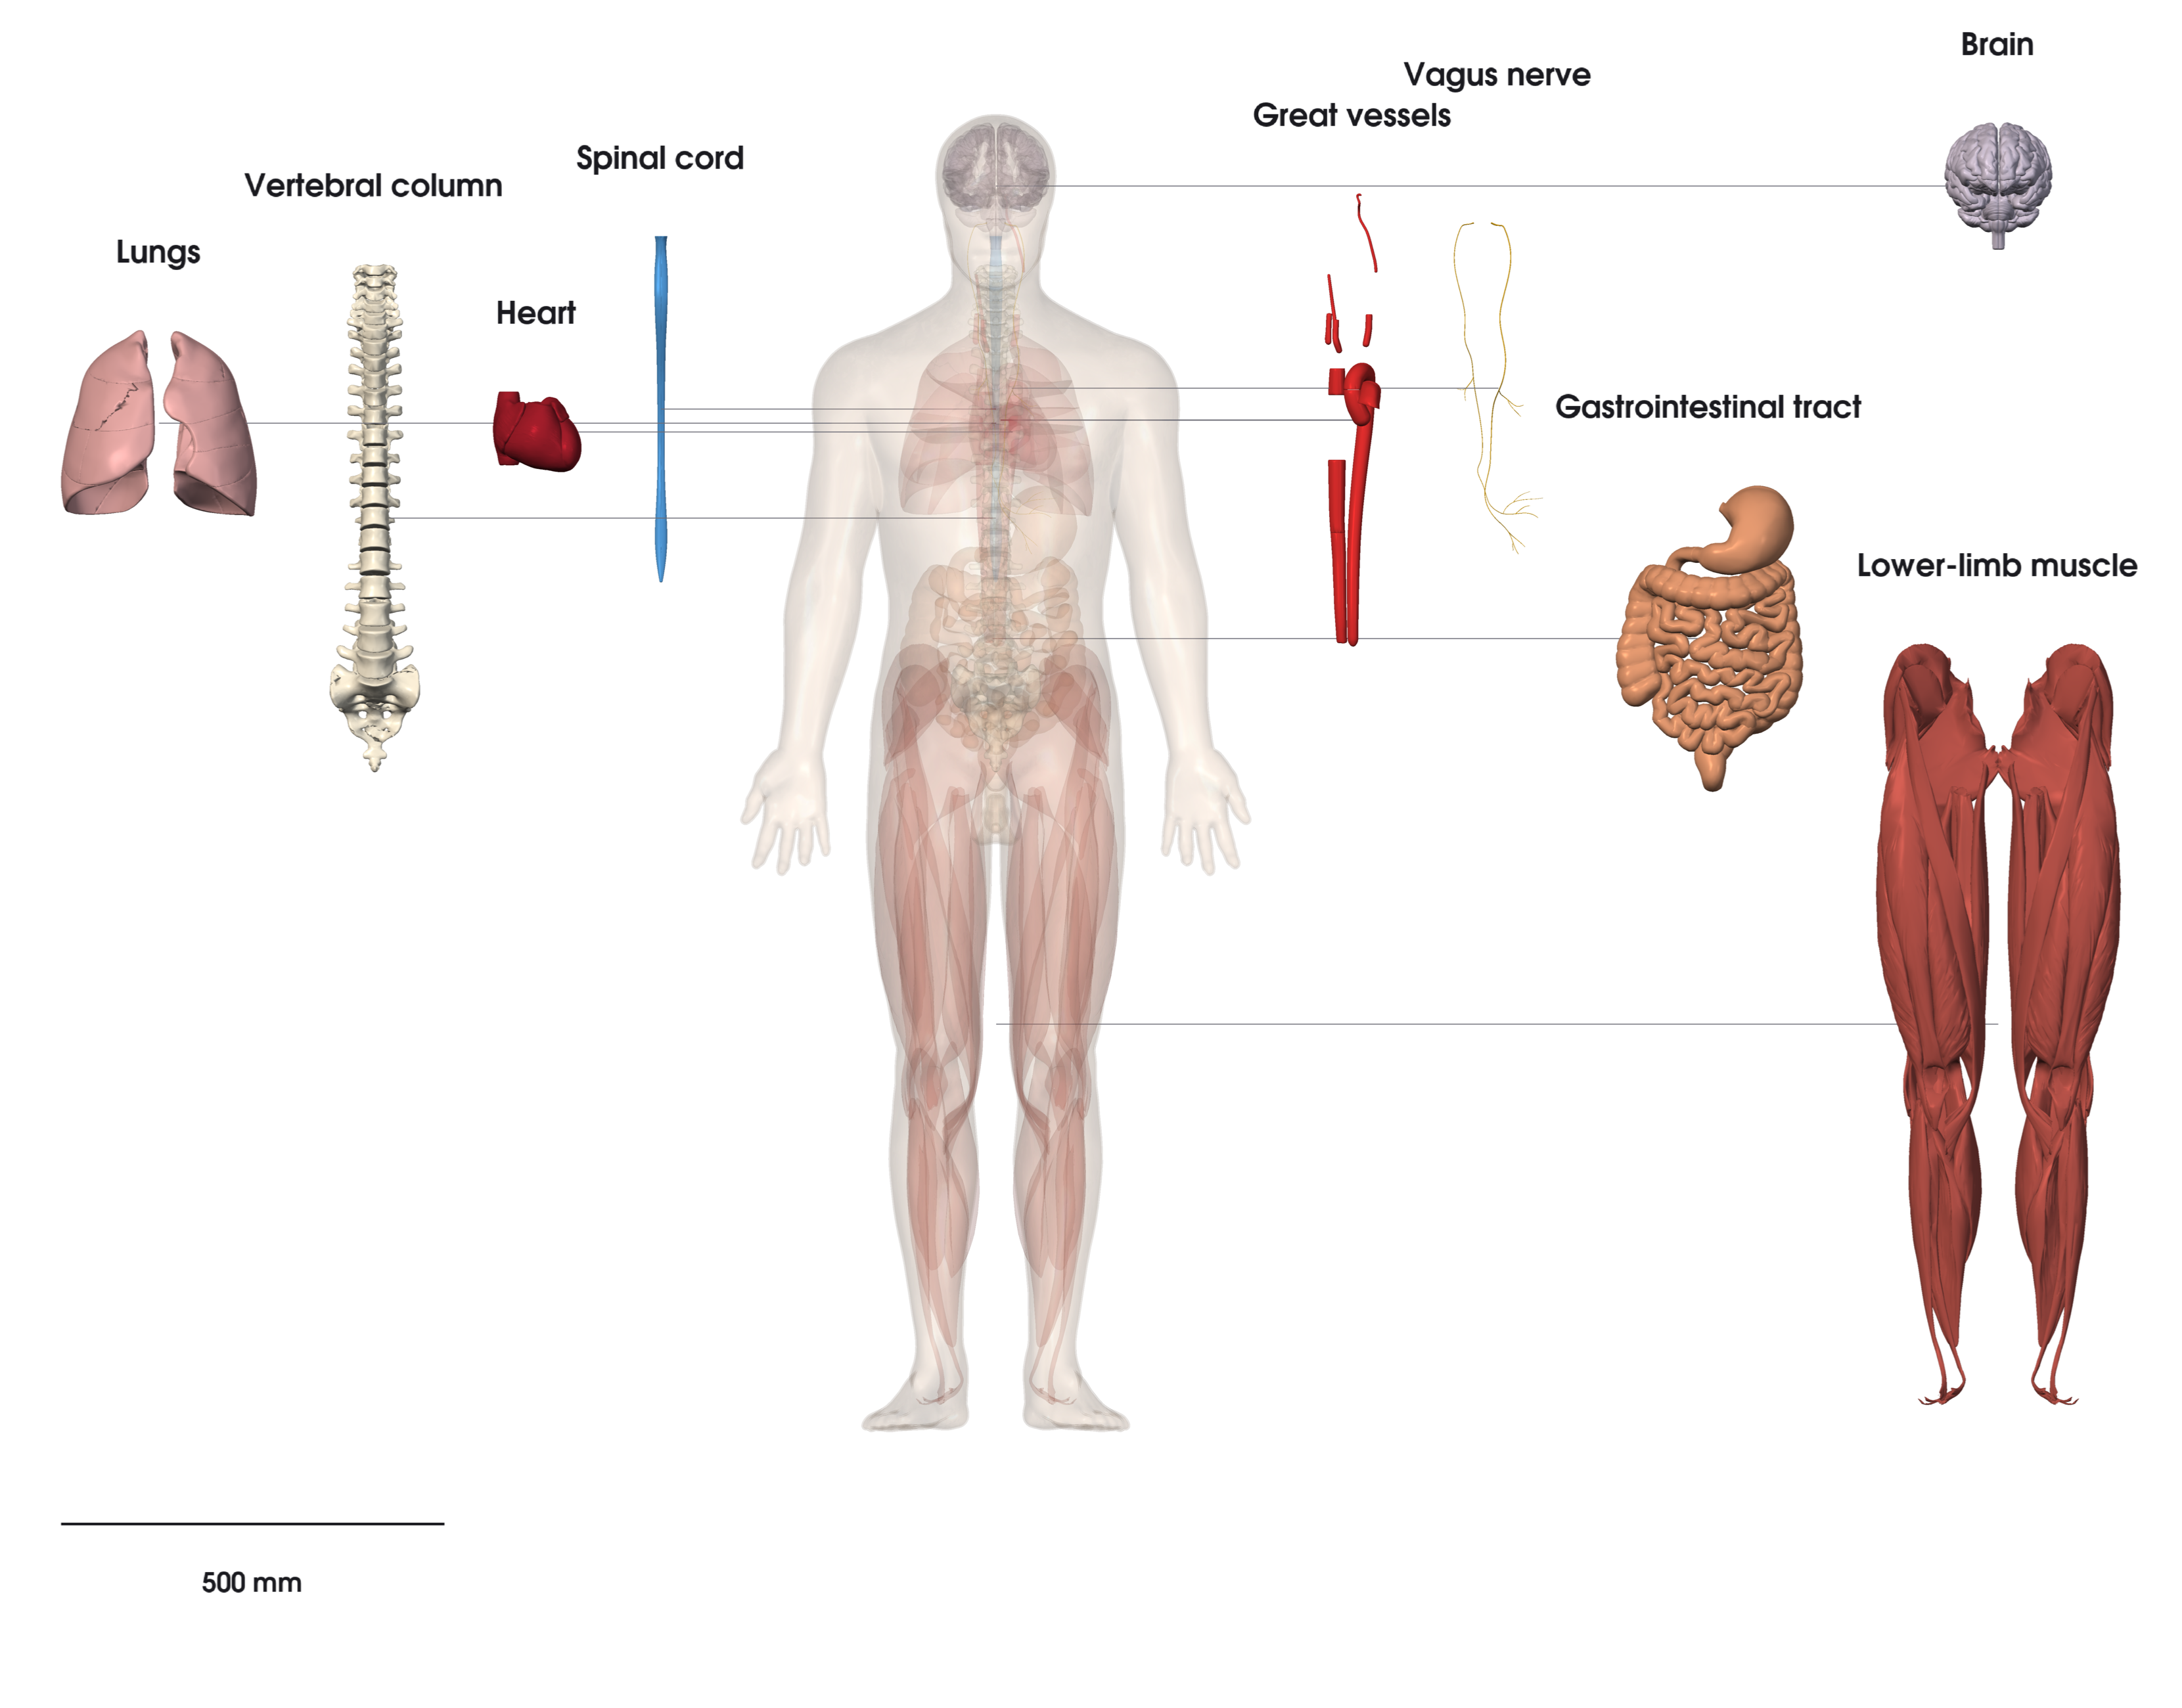
\includegraphics[width=\linewidth]{fig2_anatomy}
\caption{The iNOB anatomy contains all major tissues across
the body and can be custom-configured to include as much or as little as
required for the simulations.}
\label{fig:2}
\end{figure}

\subsection{Tetrahedral FEM
construction}\label{tetrahedral-fem-construction}

The multi-tissue tetrahedral mesh can be built on a single global voxel
grid (the voxel size, or pitch, and the margin added around the tissues,
or padding, are configurable; 3 mm pitch with 50 mm padding by default)
covering all compartments (inob.fem.cgal\_builder). Each tissue is
rasterised by the strategy appropriate to its input: convex-hull union
for compact structures such as bone, clipped to the skin envelope;
\revised{ray-traced and flood-filled for the vagus nerves, and solid-filled for
blood vessels, both with a one-voxel dilation so sub-voxel-diameter
structures remain represented on the volume grid; surface-sample
splatting with morphological closing and exterior flood-fill for muscle,
spinal cord, heart, brain and lung; and the same splatting, closing
(30 mm) and exterior flood-fill for the skin, keeping the largest
connected component and closing internal cavities,}
which accommodates anatomical openings (mouth, nostrils) for which
simple interior fills fail. Tissues are composited into a single
labelled image, painted outermost-first according to the
configuration's tissue ordering, so that inner labels
overwrite outer; CGAL Mesh\_3 is then invoked through iso2mesh.cgalv2m
(the maximum surface-element radius, radbound, and the maximum element
volume are configurable; 2.5 voxels and 20 cubic voxels by
default). The Joe-Liu mean-ratio quality (Liu \& Joe, 1994) (a
normalised tetrahedron shape measure equal to 1 for a regular
tetrahedron and tending to 0 for degenerate slivers) is gated at a
configurable minimum (minimum 0.05 by default; inob.mesh.quality). In the
default whole-body build the worst element has a mean ratio of 0.099 and
the median is 0.585, so the gate never binds and its value does not
affect the results. Mesh size, element count and per-tissue
conductivities depend on the target structure and configuration;
isotropic, frequency-independent conductivities are assigned per tissue
from the IT'IS Database (v4.1) or user-supplied values
(Gabriel et al., 1996; Haueisen et al., 2002).

\subsection{Magnetometer and surface-electrode
arrays}\label{magnetometer-and-surface-electrode-arrays}

A magnetometer array, whose sensor spacing, number of measurement axes,
stand-off from the skin and noise level are all user-specified, can be
generated by inward-radial cylindrical raycasting against the skin
surface (inob.sensors.triaxial). In plain terms, a virtual cylinder is
wrapped around the body, rays are cast inwards from evenly spaced points
on it, and a sensor is placed where each ray first meets the skin,
displaced outwards by the stand-off distance. Cylinder radius, axial and
angular spacing, stand-off distance and the glancing-hit rejection angle
are all configurable; by default the cylinder radius is 0.75×
max(X-extent, Y-extent), axial and angular spacing are matched at 30 mm,
hits are offset by a 10 mm stand-off along the outward normal
(approximating the skin-to-sensitive-volume distance of wearable OPMs),
and glancing hits (\textgreater90° between ray and outward normal) are
rejected\revised{; the default array covers the upper 45\% of body height, giving
2,730 positions and 8,190 channels}. Each surface hit carries either a single radial axis or three
orthogonal coil orientations, in a canonical FieldTrip grad layout.
Here, radial is defined as the \revised{outward} skin normal at the point where the
sensor's ray meets the skin, and the two tangential axes
are fixed relative to the body's superior (z) direction.
The single-axis option represents any single-axis magnetometer, with
sensor type captured through the stand-off and noise level; in the
triaxial case all three axes are simulated so that the optimum sensitive
axis can be identified. Users may instead supply their own sensor array
(for example, the FieldTrip grad structure of an existing system), in
which case the leadfields are computed for those positions and
orientations. Gradiometers are not implemented as a separate sensor
type, but can be represented as the difference of two coil leadfields in
a user-supplied array of coil pairs. For surface electrography, a
configurable electrode paddle or grid (inob.sensors.electrodes; contact
count, geometry and pitch set by the configuration) is placed over the
target structure's projection onto the skin; a dense
Poisson-disk whole-body array can additionally be generated for
placement sweeps across the entire body surface.

\subsection{Forward solves with
DUNEuro}\label{forward-solves-with-duneuro}

Both leadfields (MG and EG) can be computed by DUNEuro 2.10 (Python
bindings via duneuropy). The volume conductor uses mm-mode (\(\sigma\) in S/mm)
under the configured conductivity assignment. The MG path
(inob.forward.solve) attaches OPMs as point coils and uses the
transfer-matrix API (computeMEGTransferMatrix, then applyMEGTransfer)
for three orthogonal moments per source. Solver settings (CG,
reductions, SIPG scheme, integration order, subtract\_mean and
post\_process\_meg) are configurable, with defaults of reduction
10\textsuperscript{−10} and integration-order add 5. The EG path
(inob.forward.eeg) attaches electrodes with the closest-subentity-centre
realisation (codims = 1), uses computeEEGTransferMatrix and
applyEEGTransfer, and common-average references the surface potentials.
Source positions are sampled at a configurable spacing along the target
structure's polyline, by Z-slab averaging of the
corresponding tissue's tetrahedral centroids
(inob.sources); the resulting number of sources depends on the
structure's extent and the chosen spacing. Output is
scaled to \(\text{fT }\text{(nA·m)}^{- 1}\) (MG) and
\(µV\ \text{(nA·m)}^{- 1}\) (EG). Because DUNEuro's raw
output is not in these units by default, a calibration procedure was
applied, described in the next section.

\subsection{Calibration to physical
units}\label{calibration-to-physical-units}

\revised{Both modalities were checked against analytic sphere solutions. For
MG, the conversion from DUNEuro's mm-mode output to fT per nA·m follows
from dimensional analysis (scale factor 0.1 T per A·m), and on a
spherical test geometry the FEM MG peak agrees with the Sarvas
closed-form solution to within 2\% (\texttt{test\_meg\_sphere\_validation},
run against a real DUNEuro build); iNOB's analytic Sarvas implementation
itself matches MNE-Python's sphere model to a relative tolerance of
\(10^{-12}\). For EG, the same dimensional argument applies: in mm-mode
a unit moment is 1~A·mm \(= 10^{6}\)~nA·m and the potential is returned
in volts, so the raw output is µV per nA·m. We confirmed this
empirically (\texttt{inob.analysis.sphere\_calibration}): a
homogeneous-tissue sphere FEM (\(R = 100\) mm, \(\sigma = 0.43\) S/m,
voxel pitch 3 mm, ≈4,800 elements) was meshed identically to
production; 200 surface electrodes were placed on a Fibonacci lattice;
the EG forward was computed with a unit dipole at 50 mm depth; and both
the DUNEuro output and the Berg-Scherg analytic series were
common-average referenced before taking their per-(electrode, moment)
ratio. The median ratio was 0.975 and the least-squares ratio 1.016.
Across 12 cases (sphere radii of 80 and 100 mm, source depths of 30, 50
and 70 mm, conductivities of 0.2 and 0.43 S/m, 3 mm pitch;
\texttt{scripts/eeg\_calibration\_sweep.py}) the median ratio lay
between 0.98 and 1.03 (coefficient of variation 1.8\%), identical for
both conductivities, confirming the unit conversion. The least-squares
ratio, dominated by the electrodes nearest the source, ranged from 0.72
to 1.02; this is the FEM discretisation error of a 3 mm mesh close to a
shallow source. The Berg-Scherg reference
was itself validated against the textbook centred-dipole potential
\(3\,\mathbf{p}\cdot\hat{\mathbf{r}}/(4\pi\sigma R^{2})\), an
independent numerical Neumann solve (agreement to better than
\(10^{-6}\)) and
MNE-Python's sphere EEG model (to \(10^{-5}\)). An earlier version of
that series divided its radial terms by \(n\) and its tangential terms
by \(n(n+1)\), under-reading the potential by a factor of 0.4--0.9 and
producing an apparent calibration factor of 0.622; with the series
corrected, no empirical factor is needed, and
\texttt{EEG\_CALIBRATION\_FACTOR} = 1.0 in \texttt{inob/forward/eeg.py}.
The remaining numerical uncertainty is FEM
discretisation, which is largest near shallow sources.}

\subsection{Sarvas versus full-FEM
benchmark}\label{sarvas-versus-full-fem-benchmark}

Elongated target structures can be approximated by concentric-circle
geometry, with source-axis and sensor-axis distances (including any
sensor stand-off) set by the configuration. Each source is evaluated
against its own sphere, centred on the source of interest (at the same Z
as that source, on the structure's central axis), rather
than against a single fixed sphere shared across all sources, which
would inflate the amplitudes of the forward fields using the Sarvas
solution for distant sources (inob.analysis.sarvas\_compare); the axis
position is estimated as a weighted average of nearby bone tetrahedral
(tet) centroids and the source-polyline position within each
source's Z-band. For each (source, coil) pair the FEM
leadfield is projected onto the local structure tangent and compared
with the Sarvas prediction at the same orientation and moment; 95\%
confidence intervals on the peak ratio are obtained by non-parametric
bootstrap (\(B\) = 2,000 by default). The amplification reflects
secondary-current contributions captured by Geselowitz reciprocity but
absent from any single-sphere model.

\subsection{Source model and physiological
scenarios}\label{source-model-and-physiological-scenarios}

Two kinds of neural current contribute to extracranial signals.
Postsynaptic potentials, which dominate conventional MEG and EEG, are
slow and spatially stationary and are well described by a single current
dipole. Action potentials are brief and propagate along the fibre, so
each is better described by a travelling pair of opposed dipoles (a
quadrupole-like source). Peripheral nerves and white-matter tracts such
as the dorsal columns carry action potentials with little or no local
synaptic activity, so the targets considered here are modelled as
action-potential sources. Per-fibre dipole moments follow the Hämäläinen
formulation:

\emph{Q = π·d\textsuperscript{2}·σ\textsubscript{in}·ΔV/4} (9)

where d is the fibre diameter, σ\textsubscript{in} the intra-axonal
conductivity and ΔV the action-potential amplitude. σ\textsubscript{in}
is set by the configuration (1.0 S/m canonical brain-MEG convention by
default; switchable to the peripheral-axoplasm value 0.35 S/m of Pelot
et al. for peripheral-nerve targets), and ΔV is set per fibre type
(typically 70 mV for myelinated A-fibres or 80 mV for unmyelinated
C-fibres). Conduction velocity followed Hursh's law (CV
≈ 6 m s\textsuperscript{−1} µm\textsuperscript{−1}) for myelinated
fibres and 0.5 m s\textsuperscript{−1} for unmyelinated. Physiological
scenarios (inob.physiology.scenarios) are user-defined: each specifies
an event rate, a fibre population (count and diameter distribution) and
a timing relationship to a reference event, for example phase-locked to
a cardiac cycle with jitter, or to a respiratory cycle at 6 breaths
min\textsuperscript{−1} (0.10 Hz), and, where relevant, separate phasic
and tonic components. The simulator (inob.physiology.simulate) generates
per-channel time series at a configurable sampling rate (fs = 10 kHz by
default) by superposing biphasic-Gaussian compound action potentials
(CAPs; AP width σ configurable; 0.5 ms by default) at the target
hot-spot; an optional propagating-CAP control traverses the full
structure polyline at fibre-diameter-dependent CV.

\subsection{Noise floors and
detectability}\label{noise-floors-and-detectability}

Per-channel noise was modelled as quadrature-summed white noise over a
30--500 Hz recording band seen through the sensor's own
frequency response (inob.analysis.snr). For OPM magnetography,
\revised{\(\sigma_{n} = 7\ \text{fT}/\sqrt{\text{Hz}} \times \sqrt{147\ \text{Hz}} = 85\ \text{fT}\)
at the sensor output, 147 Hz being the effective noise bandwidth of the
30--500 Hz band seen through the sensor's 135 Hz pole. Because that
pole passes only part of the amplitude of a compound action potential,
the noise is referred back to the unfiltered signal by dividing by the
passed fraction, which depends on the target's CAP width: 0.39 for the
vagus (0.5 ms, spectral peak 318 Hz), 0.51 for the spinal cord (0.7 ms,
227 Hz) and 0.79 for muscle (1.5 ms, 106 Hz), giving effective floors
of 217, 166 and 108 fT,} against which unattenuated signal amplitudes are
compared (QuSpin Gen-3, QZFM-3; the Gen-2 value of
\(\text{15 fT/}\sqrt{\text{Hz}}\) is available for comparison). For
HD-EG, the amplifier term (\(0.1\ µV/\sqrt{\text{Hz}}\)) was summed in
quadrature with the Johnson voltage noise of the skin contact,
\(v_{n}\  = \ \sqrt{4k_{B}T\ R}\), at T = 310.15 K and R = 10 kΩ
(≈\(0.013\ µV/\sqrt{\text{Hz}}\)), giving
\(\sigma_{n}\  \approx \ 2.19\ µV\). The Johnson term is small compared
with the amplifier noise, so the assumed temperature (configurable) has
a negligible effect on this floor. Per-source signal amplitude was taken
as the per-source peak for MG (largest response over channels and over
the three orthogonal source moments), and as the largest bipolar
difference across contacts for EG (max − min), the latter because the
surface potentials are common-average referenced and a single-channel
amplitude would be reference-dependent. The same sensor bandwidth is
applied to the signal as to the noise, so a narrower analysis band
attenuates the compound action potential as well as the noise floor: for
a 0.5 ms CAP, whose spectrum peaks near 318 Hz, a 135 Hz single-pole
(first-order) low-pass filter passes roughly 39\% of the waveform
amplitude (an amplitude rather than power ratio: 1/√(1 + (318/135)²) ≈
0.39). \revised{The reductions in signal and in noise do not cancel: a sensor with a
1 kHz bandwidth, measured over the same 30--500 Hz band, would have an
effective vagal floor of 153 fT, so the 135 Hz pole costs a factor of
1.42 in noise and about 2 in trials-to-detect.} Trials-to-detect at the Rose
criterion (SNR = 3) was inverted from \(\text{SNR ∝ }\sqrt{N}\) for
white uncorrelated noise. Spatially correlated environmental noise could
inflate trials-to-detect, and spatial filtering (for example, LCMV/SAM
beamforming) could reduce it; neither is modelled here. Both noise
floors are instrument-only: they exclude environmental interference and
movement artefact for OPMs, and physiological noise (EMG, ECG and
background EEG) for electrodes. All trial counts reported here should
therefore be read as holding under instrument-limited noise.

\section{Worked examples}\label{worked-examples}

The following worked examples demonstrate what the package can do, which
inputs can be changed, and what is returned in each case. The three
targets were chosen to span the range of problems iNOB is designed for:
the spinal cord, a deep source encased in low-conductivity bone; the
cervical vagus, a superficial nerve with no intervening bone; and the
neck muscles, a strong, anisotropic, volume-filling source that is more
often treated as interference than as signal. In each example the same
source-sampling rule, sensor arrays (a triaxial OPM array wrapped around
the body, a 32-contact surface-electrode paddle over the target, and a
dense whole-body electrode array for coverage comparisons; Section 3.3)
and noise floors (Section 3.8) are used, so that differences between
examples reflect anatomy and physiology rather than differently assumed
inputs. All of these inputs can be changed: source spacing
(forward.source\_spacing\_mm), array geometry and number of sensors,
sensor stand-off, noise levels, the electrode reference and the source
orientation are configuration or command-line options. Positions are
given in the body frame used throughout iNOB, in which z is superior and
−y is anterior. Each example first compares the analytic and full-FEM
forward solutions, then reports the sensor-level amplitudes and
trials-to-detect for each modality.

\subsection{The spinal cord}\label{the-spinal-cord}

The spinal cord is a key component of the central nervous system, and is
involved in a number of critical neural processes, such as pain
perception and breathing control. Due to the geometry of the torso, the
spinal cord is a clear example of a case where the standard spherical
assumptions which might be made for source imaging in encephalography
break down (cite George's paper). Here we demonstrate how iNOB can be
used to flexibly generate ESG and MSG leadfields under different source
and sensor assumptions.

The spinal cord is taken first because it is where the full multi-tissue
FEM differs most from an analytic approximation. Spinal cord sources lie
deep beneath the body surface, their evoked fields are weak (about 14
times weaker than those of peripheral nerves), and they are embedded in
a complex, low-conductivity volume of vertebral bone. The section works
through four questions in turn: how well a single-sphere approximation
compares with the full FEM for the spinal cord; what signal is observed
if the entire cord is synchronously active; what signal results from an
arguably more physiologically realistic (cite Japanese work) travelling
volley instead; and whether wider electrode coverage can close the gap
in trials-to-detect between surface electrodes and OPMs. The forward
solution for a single unit dipole on the cord axis is shown in Figure 3.

We first compare the single-sphere (Sarvas) approximation with the full
FEM, because an analytic model is fast and less sensitive to errors in
the anatomical model, and so is worth using wherever it is adequate. The
cord runs inside the vertebral canal, encased in bone, and its
calibrated source strength of 5.11 nA·m is small compared with the vagus
(70 nA·m) and muscle (10--1,000 nA·m). This encasement means that a
homogeneous single sphere is a poor approximation for the spinal cord.
As bone is a low-conductivity medium compared with the surrounding
tissues, the sharp conductivity contrast drives strong return (volume)
currents, which heavily influence the field that the sensors measure.
The single-sphere solution has no way to represent bone forcing return
currents through the surrounding soft tissue, and its prediction
diverges sharply from the FEM's, whose peak field comes
out \revised{4.34× higher (95\% CI 4.25--4.41, B = 2,000)} at the same source strength.

The next question is what happens if the whole cord is modelled using
the simple Sarvas method, as one synchronous generator, the simplest
possible source assumption. Firing all 91 modelled segments in phase
predicts \revised{5.32 pT (OPM) and 9.66 µV (ESG) at the C6/C7 level}, both detectable in a
single trial. This provides an upper bound for expected M/ESG signals
but ultimately is unrealistic: the modelled cord spans \revised{477 mm}, meaning
an ascending volley takes approximately 8.1 ms to traverse it at 59 m/s, so the
time resolution of electrophysiological imaging is sufficient that such
travelling sources would not appear synchronously. Collapsing them into
one dipole inflates the OPM amplitude by \revised{57×} over the true
travelling-volley estimate, making this case a naïve upper bound rather
than a realistic estimate.

Restricting the question to a single dipolar generator entering at \revised{C6/C7}
gives a more realistic pair of estimates. Summing the volley into one
stationary segment gives \revised{208.5 fT / 6 trials} (OPM) and \revised{0.535 µV / 151
trials} (ESG). Altering our source assumptions to instead represent a
single wavefront travelling rostrally along the spinal cord at 59 m/s
reduces these values to \revised{92.8 fT / 29 trials and 0.159 µV / 1,709 trials}. \revised{Both electrode estimates are within a clinical averaging budget: the
stationary one below and the propagating one inside the
500--2,000-average somatosensory evoked potential (SSEP) range. Which is
closer to a real recording depends on an assumption this model cannot
settle: a genuine SSEP also carries a postsynaptic dorsal-horn component
that does not travel. What does not depend on that unresolved question
is the modality gap at a fixed cervical patch: OPM needs 25--59 times
fewer trials than the 32-contact patch under either source model, so,
under the noise assumptions used here, the OPM advantage at the patch
holds however the stationary/propagating balance is eventually
settled.} This runs counter
to empirical experience, in which ESG is often easier to observe at the
sensor level than MSG, and underlines that these estimates depend
strongly on the assumed noise levels and source model.

\revised{Given how far EG lags OPM at a fixed cervical patch, we next ask whether
wider electrode coverage closes the gap. It largely does. With the same
source models, the 1,000-contact whole-body array reaches SNR 3 in 45
trials for the stationary source (0.987 µV) and 48 for the ascending
volley (0.947 µV), against 1,709 for the 32-contact patch and 29 for
OPM, leaving OPM ahead by a factor of only 1.7 in trials. This is
consistent with the empirical experience above. Along the cord, the
whole-body array's best single contact sees a median of 40 times the
patch's signal (range 2.9--170×). Most of that advantage comes from the
rostral end of the cord: at source \#90 (z = 1482 mm, at the C1 level, just below the skull base)
the whole-body coupling is 1.21 µV per nA·m against 0.19 at C6. A volley
reaching the head--neck junction drives a head-versus-trunk potential,
the same far field that clinical SSEP recordings capture as the P14 with
a non-cephalic reference. The result therefore depends on where the
modelled cord ends, and should be read as a statement about that far
field rather than about electrode coverage as such.} \revised{Extending coverage beyond the cervical patch also recruits
progressively larger muscle groups; a single motor unit near C7 already
exceeds the cord volley by roughly 300--950×, each measured on its own cervical
paddle (150
µV against 0.16--0.54 µV), so each added channel brings muscle artefact
as well as sensitivity, an argument the muscle example below makes in
full.}

\revised{The same machinery answers practical questions about the sensors
themselves. Holding the source at the default cervical position
(Q = 5.11 nA·m) and repeating the DUNEuro solve at each sensor
stand-off (\texttt{scripts/sensor\_sweep.py}), the best channel of the
triaxial array gives 43.7 fT per nA·m at 6.5 mm, 40.7 at 10 mm, 31.4 at
20 mm and 24.6 at 30 mm, that is, 223, 208, 160 and 126 fT. Against the
166 fT floor of a Gen-3 sensor (7 fT/\(\sqrt{\text{Hz}}\)) these need
5, 6, 10 and 16 trials to reach SNR 3; against the 356 fT floor of a
Gen-2 sensor (15 fT/\(\sqrt{\text{Hz}}\)), 23, 26, 44 and 72. Moving the
array from 10 to 20 mm off the skin costs 23\% of the amplitude and
about 1.7 times the trials, whereas moving from Gen-3 to Gen-2 sensors
costs about 4.5 times the trials. A single-axis radial array needs
about 2--4 times more trials than a triaxial one (radial-only peak 21.0
fT per nA·m at 10 mm).}

\begin{figure}[htbp]
\centering
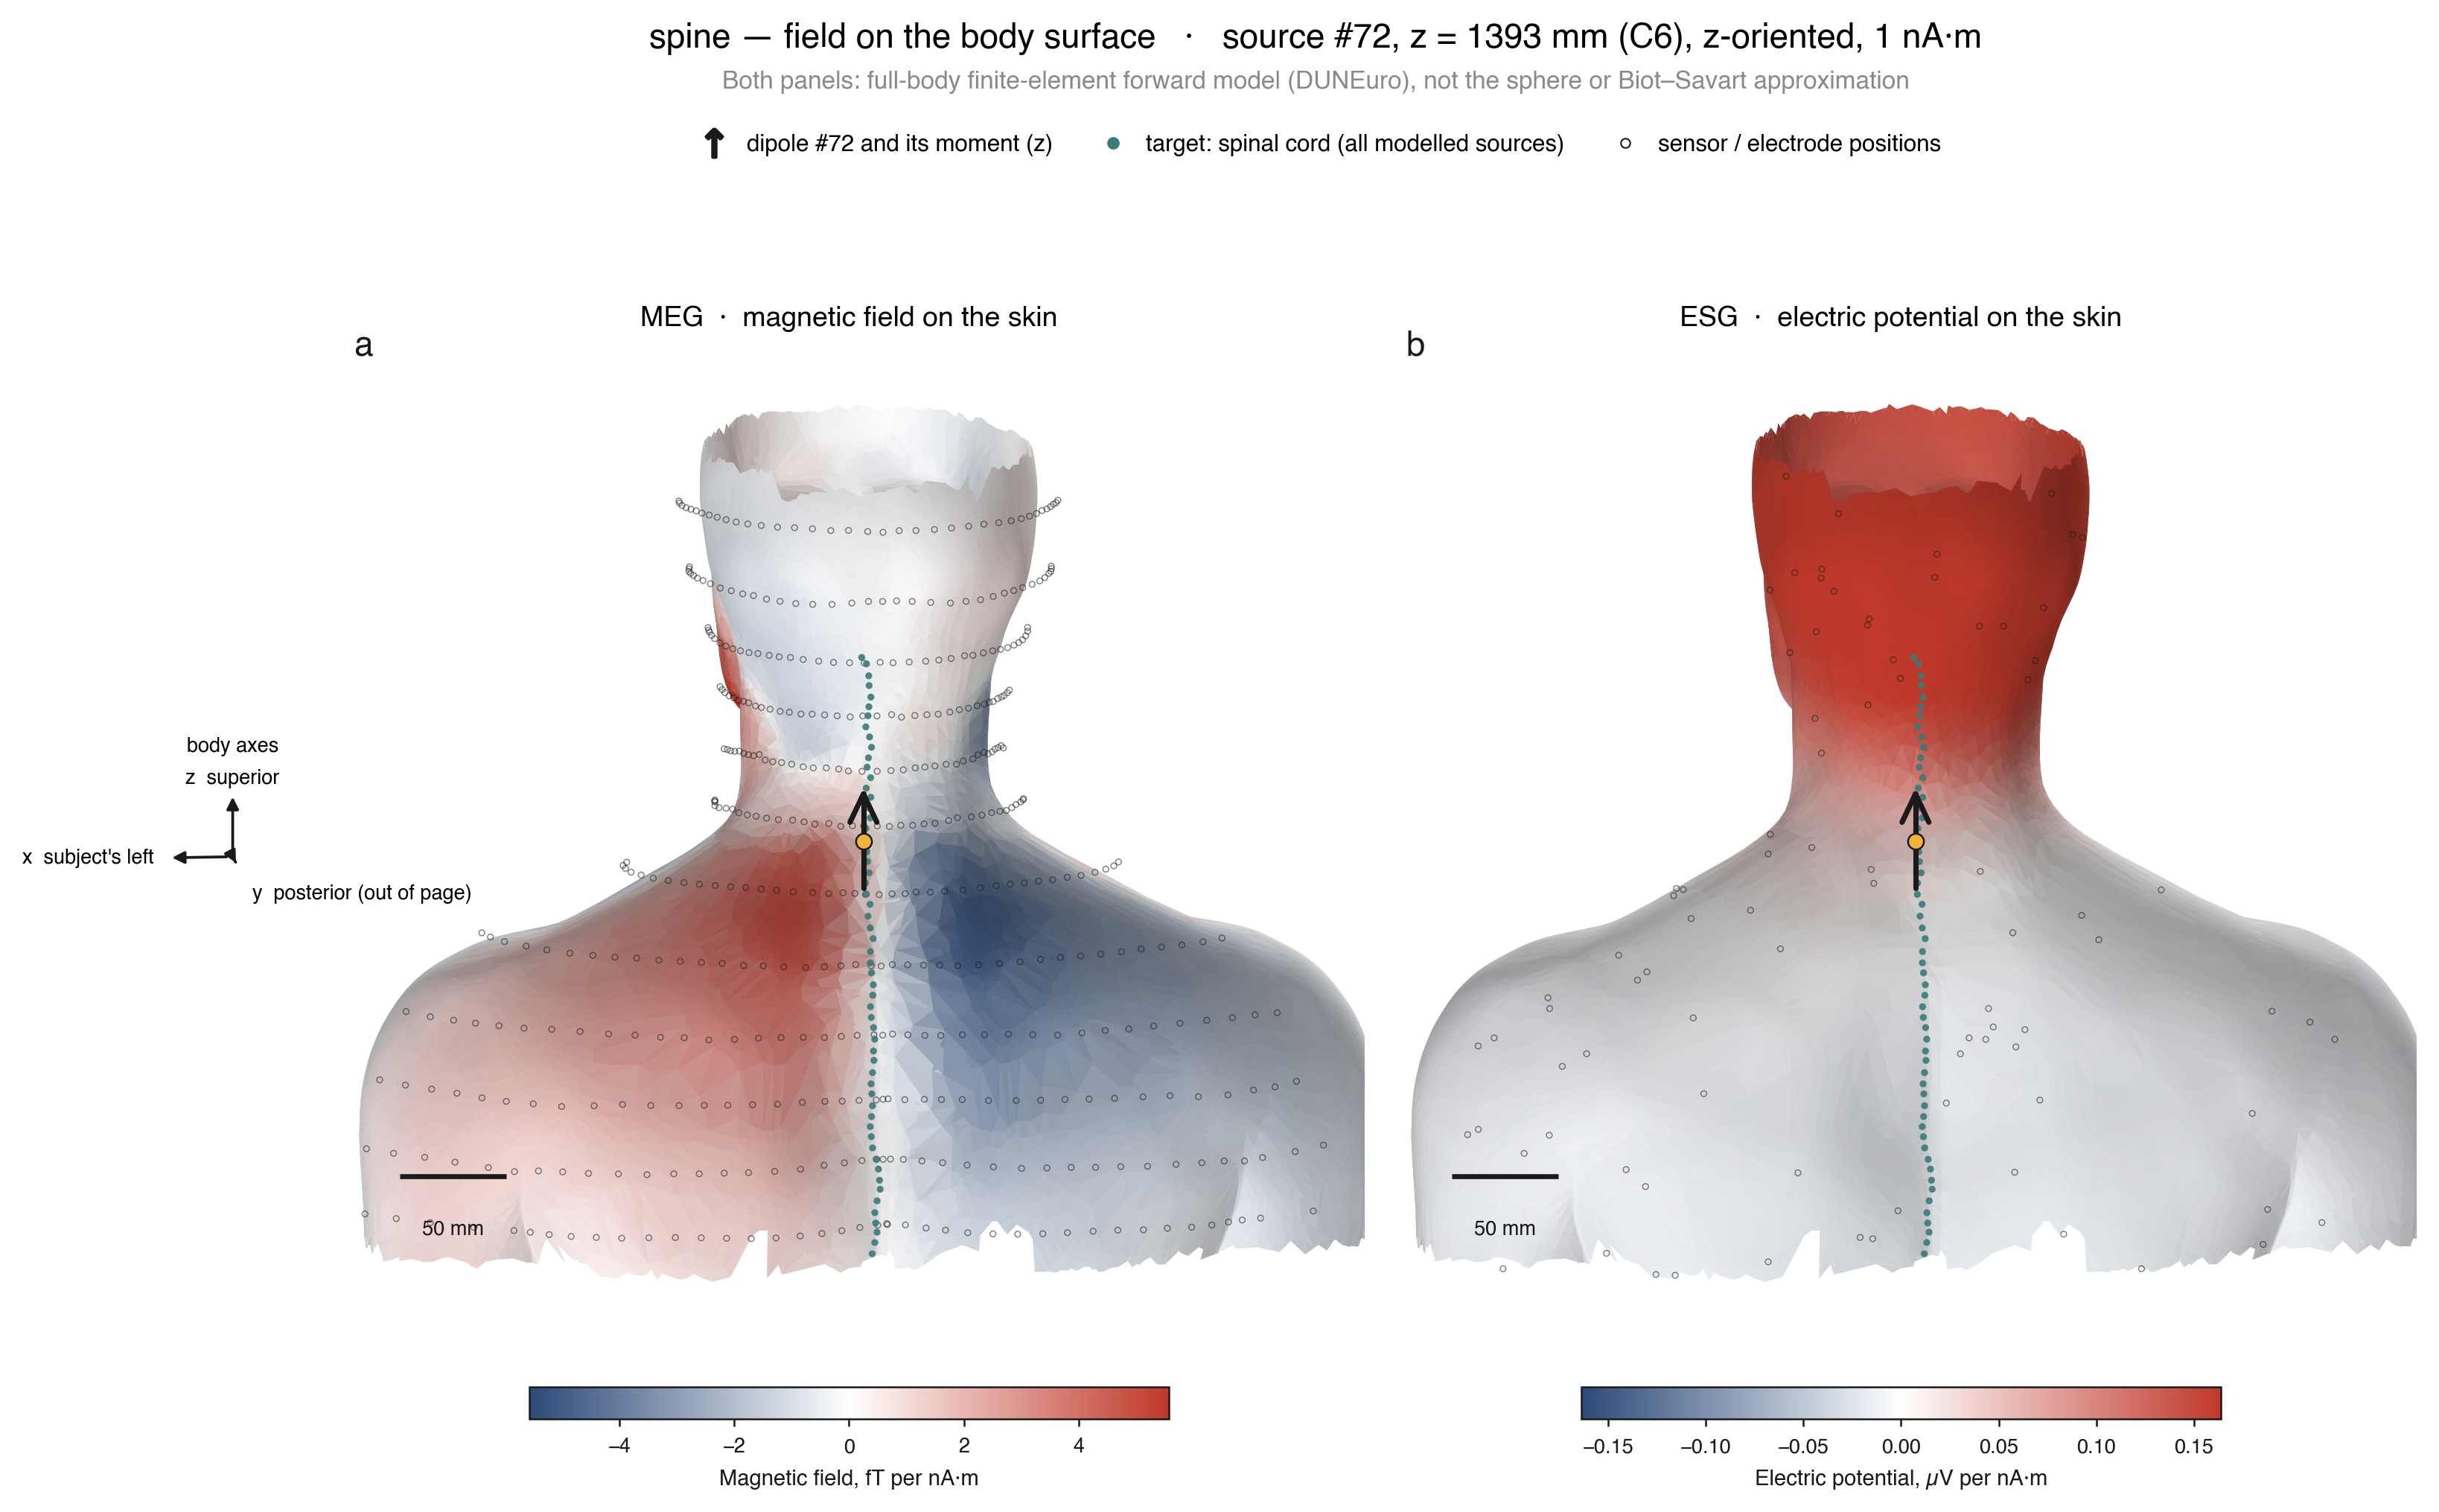
\includegraphics[width=\linewidth]{fig3_spinal_cord}
\caption{Spinal cord forward solution. Fields are shown for a
single z-oriented unit dipole (1 nA·m) on the cord axis at \revised{z = 1393 mm,
level C6 (source \#72), drawn as an arrow along its moment in both panels;
teal dots mark all modelled cord sources and open circles the sensor and
electrode positions}. (a) Radial
magnetic field on the skin, interpolated from \revised{2,730 triaxial OPM
positions at 30 mm pitch}. (b) Surface electric potential on the same
skin, interpolated from \revised{1,000 whole-body electrodes (\textasciitilde20
mm mean contact spacing)}, common-average referenced. Both panels share
mesh, camera, orthographic projection and scale (bar: 50 mm): \revised{the
magnetic field divides the neck left from right about the midline, while
the potential divides it head from trunk, the two patterns roughly
orthogonal.} Skin further than 1.6 × the array spacing from the nearest
sensor is left unpainted. Colour scales are symmetric about zero,
clipped to the 98th percentile of the measured surface \revised{(±5.6 fT per nA·m
in a; ±0.16 µV per nA·m in b)}, and are given beneath each panel.}
\label{fig:3}
\end{figure}

\subsection{The cervical vagus}\label{the-cervical-vagus}

In contrast to the spinal cord, nothing bony sits between the vagus and
a sensor on the neck, so the analytic sphere remains defensible here
where it fails for the cord: the homogeneous approximation is not being
asked to represent a shell that forces return currents through soft
tissue. The full FEM still runs, but for the vagus it serves to confirm
the approximation. The corresponding forward solution is shown in Figure
4.

It also has the clearest experimental motivation, since direct vagal
recording currently requires an invasive cuff, intraneural electrodes or
ultrasound-guided microneurography. The forward model places 88 dipoles
along the nerve across \revised{z = 1068--1502 mm, at the same 5 mm axial spacing
as the cord (88 dipoles for the vagus, 91 for the cord)}, so any
difference between the two examples is geometry rather than a
differently assumed source. The question posed here is the one set out
in the Introduction: for a physiologically realistic source, what would
an OPM array and a surface-electrode paddle on the anterior neck
measure, and how many averaged trials would each need to see it? The
section takes this in order: first the comparison of the MG and EG
forward solutions with their analytic references (Sarvas and
Berg-Scherg, respectively), then the leadfield amplitudes each modality
achieves, then the resulting trials-to-detect, and finally whether
electrode placement rather than physics is what limits the electrical
measurement.

\revised{As described in Section~\ref{calibration-to-physical-units}, the FEM MG
peak field agrees with the Sarvas peak to within 2\% on a spherical test
geometry, and the median EG ratio to the Berg-Scherg series lies within 3\%
of unity across radius, depth and conductivity, with no empirical
calibration factor.} On the cervical
anatomy, the full multi-tissue FEM exceeds the homogeneous-sphere
simulation at the best-aligned coils (those with the largest response)
by a peak factor of \revised{2.11 (95\% CI 1.80--2.30; B = 2,000 bootstrap)},
consistent with secondary-current contributions at conductivity
interfaces; rescaled to full A+C-fibre summation
(\(\text{Q = 70 nA·m}\)) the Sarvas peak is \revised{3.0 pT}, within the 1--4 pT
range reported by Bu et al. (2024). The maximum MG leadfield at the OPM
array is \revised{190.7 fT per nA·m}, against
\revised{0.190 µV per nA·m for the best single contact (0.248 for the
best pair)} at the cervical electrode paddle.
Coupling is strongly position-dependent along the nerve: the
best-coupled source returns \revised{190.7} fT per nA·m, the median across the
nerve \revised{29.7} and the worst \revised{11.3}. That \revised{17-fold} spread matters in practice,
since trials-to-detect varies by roughly two orders of magnitude from
one end of the nerve to the other\revised{ (1--133 trials at 5 nA·m)}. Above z ≈ 1300 mm (the T4 level), where the array
provides coverage, the cervical vagus \revised{needs 1--10 trials at 5 nA·m}, while the same source at mid-thoracic level needs tens of
averages. \revised{A 1,000-contact whole-body array improves the best-pair amplitude
over the 32-contact paddle by 1.6× at the patch-centred source (at most
2.8× anywhere along the nerve), giving about 2.5 times fewer trials (27 to
about 11 at 5.11 nA·m, against the OPM's 3),} and a tissue-path
analysis confirms no bone lies between the anterior cervical vagus and
the skin: neither placement nor bone shielding is limiting. The limiting
factor is the \(\frac{1}{r^{2}}\) attenuation of the surface potential
across approximately 50 mm of conductive soft tissue, which \revised{is only
partly recovered by electrode repositioning}.

The vagus can be treated as one stationary generator, and this is where
it parts company with the cord. Carotid-sinus baroreceptor afferents are
localised to the cervical bundle, so the event propagates over a \revised{45 mm}
active segment rather than the whole \revised{531 mm} of modelled nerve. At a mean
fibre conduction velocity of 47.3 m/s that is a \revised{0.96 ms} transit against
a 0.50 ms action-potential width; the two are comparable, so the lumped
approximation holds, with \revised{a 6\% peak error}. Modelling the same
200-fibre event as a travelling wavefront gives \revised{11.69 fT} against the
stationary model's \revised{10.97 fT}, a ratio of \revised{1.065}. \revised{For the vagus,
propagation is therefore a small correction, and the stationary model is
a close, slightly conservative approximation, whereas collapsing the
cord's 8.1 ms ascending volley inflates its amplitude by 57×. The two
vagal models differ more in shape than in size: the travelling
wavefront is nearly four times sharper (FWHM 0.50 ms against 1.87
ms).}

\revised{Across a 0.74--70 nA·m sweep at the patch-centred source (\#53,
z = 1333 mm, the T2 level), against a 217 fT OPM noise floor and a 2.19
µV electrode noise floor over 30--500 Hz, the OPM array needs 132 trials
at 0.74 nA·m, 73 at 1 nA·m, 3 at 5.11 nA·m and a single trial from 10
nA·m (768.2 fT, SNR 3.5); the electrode patch, taking its best contact
pair, needs 1,279, 700, 27 and 7 trials at the same strengths, and one
trial only at 70 nA·m. The patch requires 9.7× more trials at every
rung: both amplitudes scale linearly with Q and trials-to-detect as
1/Q², so the ratio is exact and independent of the assumed source
strength, and it is the one figure here that does not depend on the
eventual choice of Q. At the cord's own 5.11 nA·m anchor, the vagus
needs 3 OPM trials against 27 electrode trials. What the sweep does not
settle is which rung is real: a single 200-fibre baroreceptor burst is
0.74 nA·m, while full A+C-fibre summation is 70 nA·m. The range spans
that uncertainty rather than resolving it, and since trials-to-detect
scales as 1/Q², the choice moves the answer by two to three orders of
magnitude while leaving the 9.7× modality gap untouched.}

\begin{figure}[htbp]
\centering
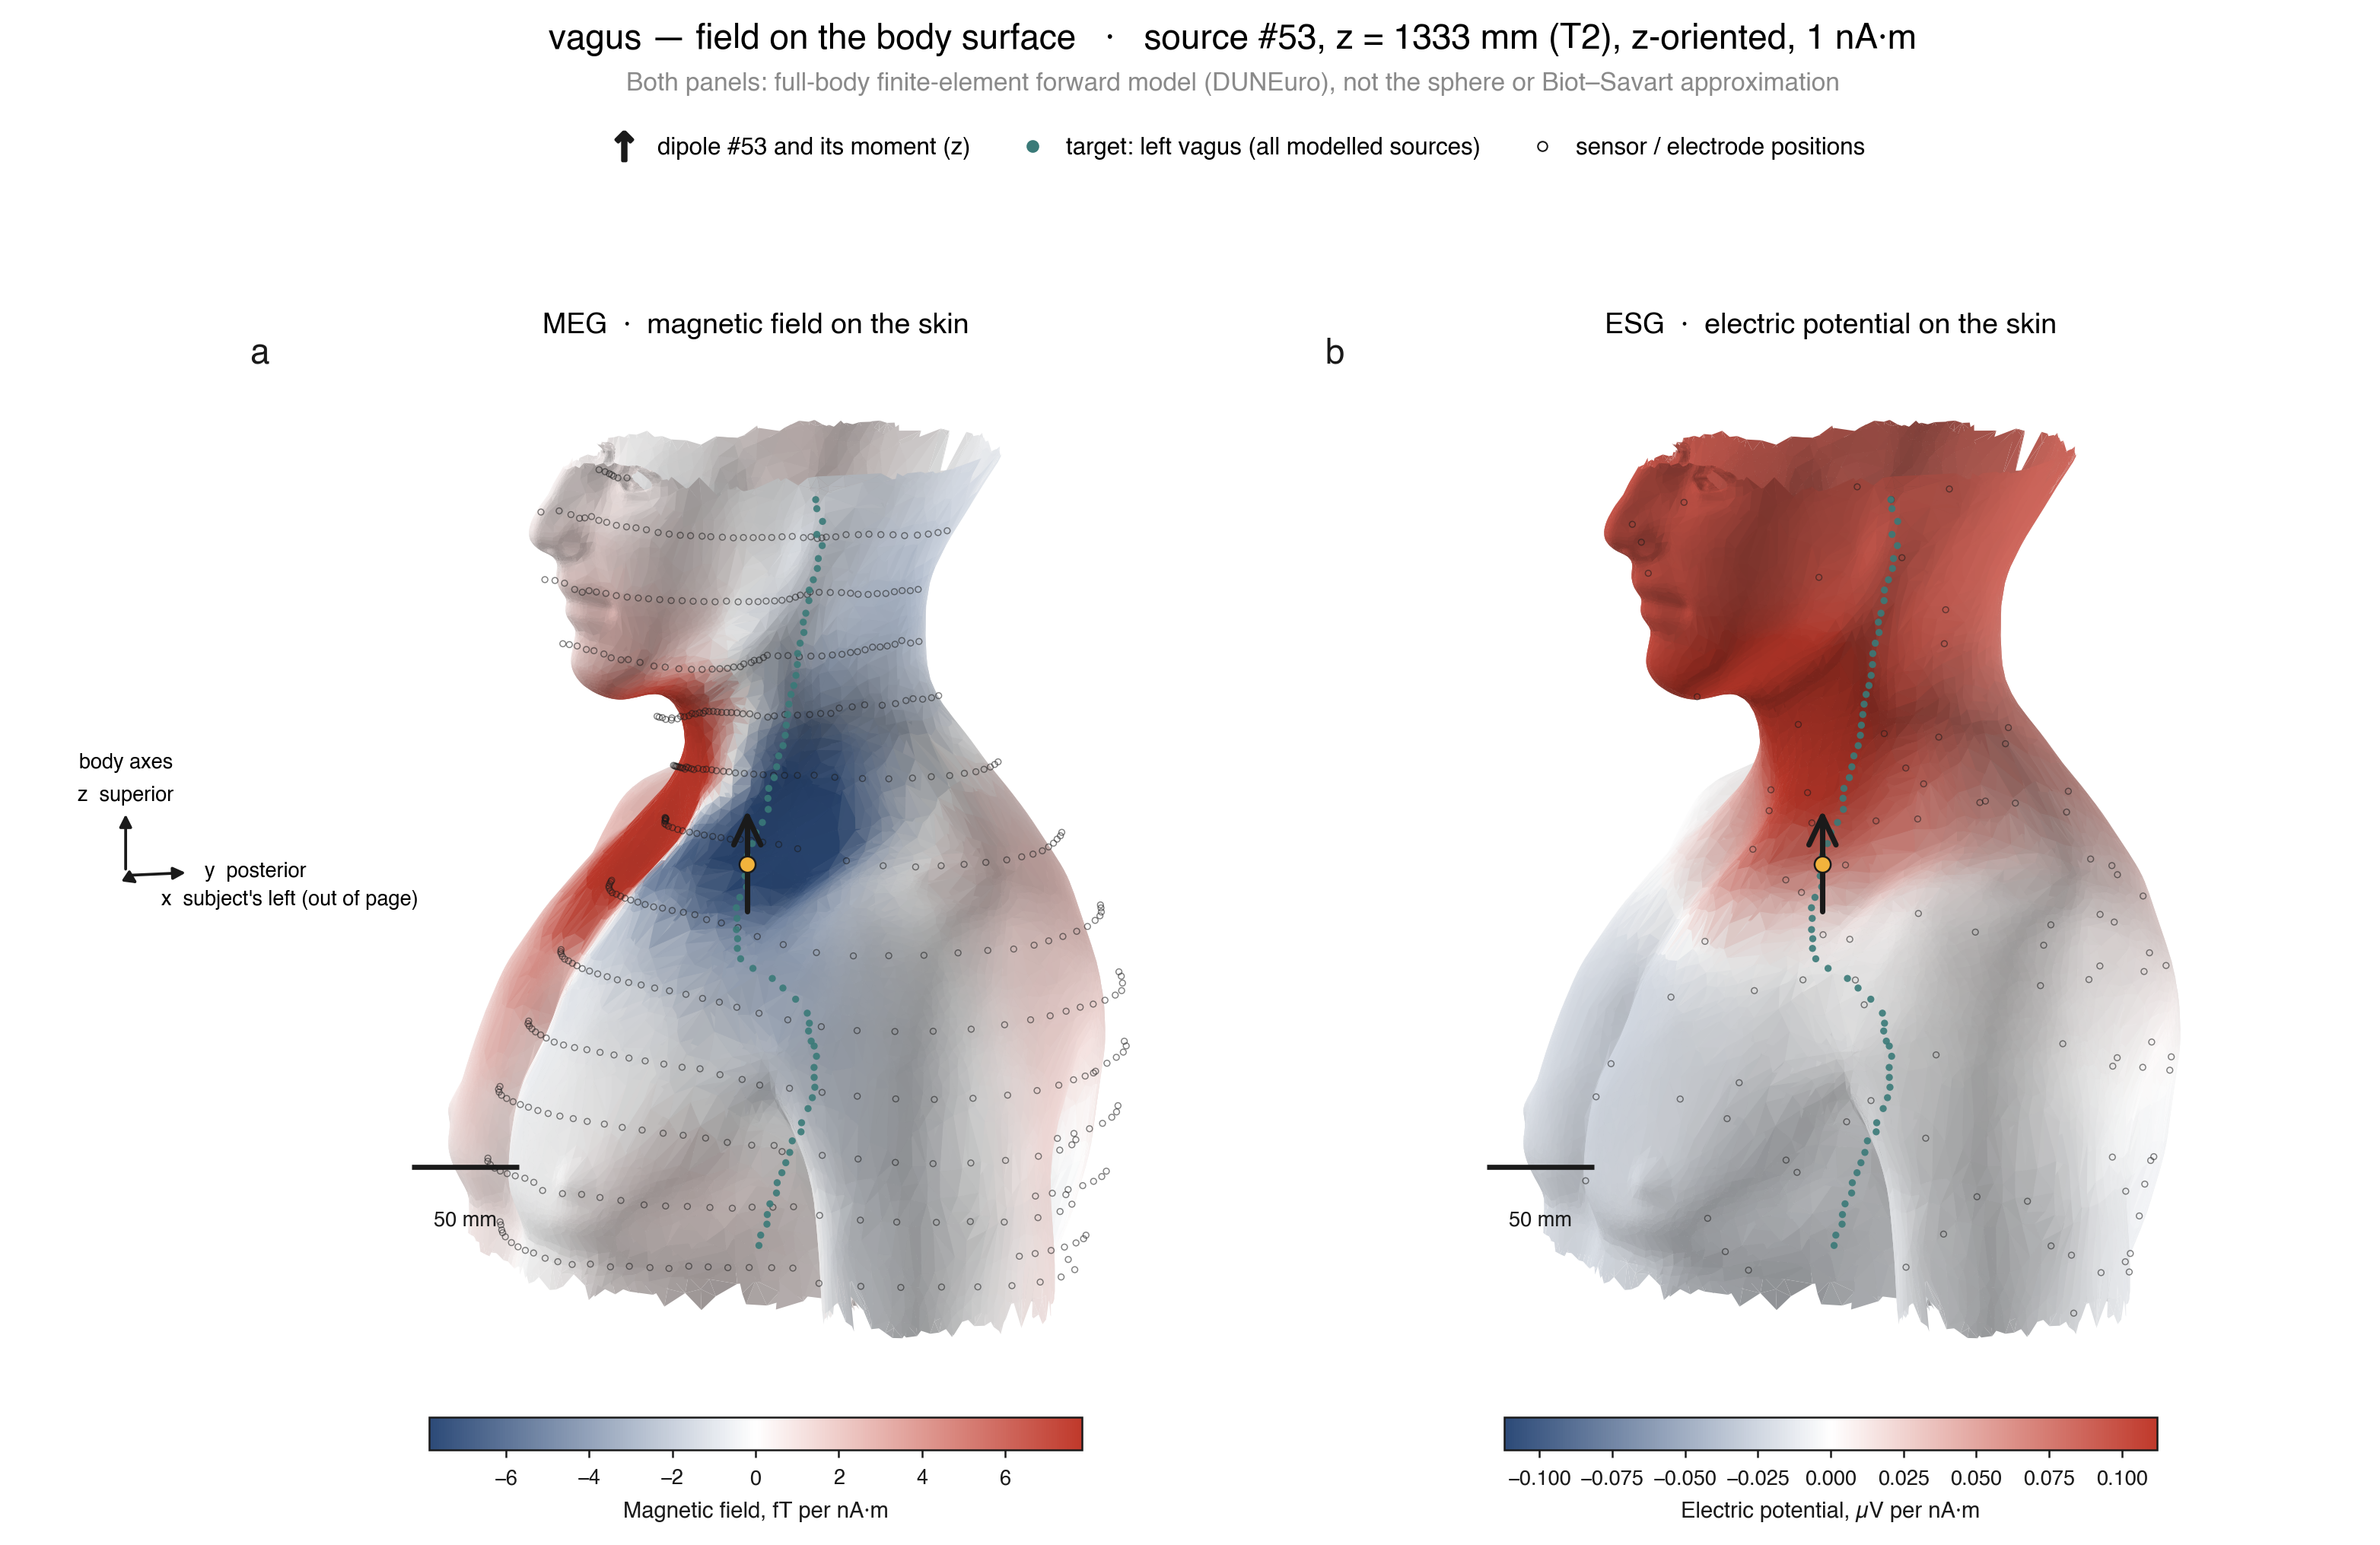
\includegraphics[width=\linewidth]{fig4_vagus}
\caption{Vagus nerve forward solution. Fields are shown for a
single z-oriented unit dipole (1~nA·m) on the left vagus nerve at \revised{z =
1333 mm, level T2 (source \#53), drawn as an arrow along its moment in
both panels; teal dots mark all modelled vagal sources}. (a) Radial
magnetic field on the skin, interpolated from \revised{2,730 triaxial OPM
positions at 30 mm pitch}. (b) Surface electric potential on the same
skin, interpolated from \revised{1,000 electrodes sampled over the whole body
(\textasciitilde20 mm mean contact spacing)}, common-average referenced.
Both panels show the same mesh in the same orthographic camera at the
same scale (bar: 50 mm), \revised{so the roughly quarter-turn between the magnetic pattern (split front
to back across the nerve) and the electric pattern (split head from
trunk) of one current dipole can be read directly.} Skin
further than 1.6 × the array spacing from the nearest sensor is left
unpainted. Colour scales are symmetric about zero, clipped to the 98th
percentile of the measured surface \revised{(±7.9 fT per nA·m in a; ±0.11 µV per
nA·m in b)}, and are given beneath each panel; the units differ by four
orders of magnitude, so the two bars are separate.}
\label{fig:4}
\end{figure}

\subsection{Neck muscles}\label{neck-muscles}

Muscle is included as the opposite extreme to the two example targets.
Where the cord and vagus test whether a signal can be recovered at all,
muscle is strong enough that detectability is never in doubt; its
interest lies instead in how it must be modelled, and in what it does to
the other two targets when it is present as interference rather than as
the signal of interest. The section first sets out the three ways the
muscle forward model departs from the nerve cases, then gives the
resulting detectability figures, and finally returns to muscle in its
role as an artefact source for spinal and vagal recording. The muscle
forward solution is shown in Figure 5.

The muscle forward model differs from the nerve targets in three ways,
all forced by the geometry. First, the sampling: the vagus and spinal
cord take one dipole per axial Z-slab, which is faithful for a thin
structure. Muscle is instead volume-filled: a regular 15 mm grid over
the muscle compartment, one dipole per occupied voxel, snapped to a
real tetrahedron centroid, giving \revised{736} dipoles across the 40 neck-muscle
meshes. The grid spacing is configurable (\texttt{forward.source\_spacing\_mm});
15 mm keeps the solve tractable, and because each muscle dipole
represents the summed activity of a volume of tissue rather than a
single fibre, a coarser grid is appropriate here than for the nerve
targets. The PCA-derived long axis of each muscle serves as a
fibre-direction proxy, but it enters the model through the conductivity
tensor rather than through the source moments: the forward solve places
three orthogonal unit dipoles at every source and detectability takes
the best-aligned of the three. The amplitudes reported below are
therefore a best-of-three-orientations bound, not a fibre-aligned
prediction. Second, we must spatially sub-sample the muscle for
computational efficiency. A 15 mm grid is far coarser than the tissue it
stands for, so each retained dipole carries the current of the whole
voxel it represents, not of one fibre. A single 60 µm fibre is about
0.25 nA·m under the Hämäläinen estimation above, but the ladder starts
at 10 nA·m (a 40-fibre motor unit) and runs to 1,000 nA·m (a whole-muscle
evoked compound M-wave). Even the bottom rung sits well above the
cord's 5.11 nA·m and the vagus's
single-burst 0.74 nA·m, and the upper rungs exceed even the
vagus's 70 nA·m full-summation figure, since Q scales as
fibre diameter squared and muscle fibres are roughly 8× bigger than
vagal A-fibres. Third, muscle is the only target given an anisotropic
conductivity: a fibre-aligned tensor with σ∥ = 0.40 S/m and σ⊥ = 0.10
S/m (Gabriel 1996; Rush 1963), one per muscle mesh and aligned to that
muscle's own axis, enabled through native options within
DUNEuro.

As expected, trials-to-detect is drastically reduced compared to the
other physiology modelled in this tool. Against noise floors of \revised{108 fT}
(OPM) and 2.19 µV (EMG) over 30--500 Hz, a single motor unit action
potential (MUAP) at 10 nA·m \revised{at the default source (\#330, z = 1375 mm, C7
level) gives 5,400 fT} on the best OPM channel and
\revised{150.3 µV} on the best contact pair of the cervical paddle sited over it,
which is SNR \revised{50} (MMG) and \revised{69} (EMG) in a single trial. Every stronger
rung is likewise single-trial detected in both modalities, so the
averaging question that dominates the spinal cord case simply does not
arise: muscle is easily detectable, and the interesting questions are
about localisation and separability instead. The amplitude argument on
which this rests, Q ∝ d² with a motor unit firing tens of large fibres
near-synchronously, is also the model's main limitation.
The model treats the MUAP as a single synchronous fibre volley, an
evoked-M-wave analogue with no motor-unit recruitment, firing-rate or
MUAP-shape model. It represents the magnitude argument well, although it
makes no modelled assumptions about voluntary contraction.

The question that this work seeks to address is the detectability of an
electrophysiologically active medium. Muscle activity is simply so large
that it is always detectable. Often, muscle activity acts as
interference rather than the signal of interest, obscuring the spinal
cord and vagus nerve, for example. For this reason, the detectability
result is not surprising. \revised{The modality comparison for the
nerve targets rests on the earlier worked examples: a 32-contact
electrode patch needs 59 times more trials than OPM for the ascending
spinal volley and 9.7 times more for the vagus, while a 1,000-contact
whole-body array narrows those gaps to 1.7 and about 3.9 times.}

\begin{figure}[htbp]
\centering
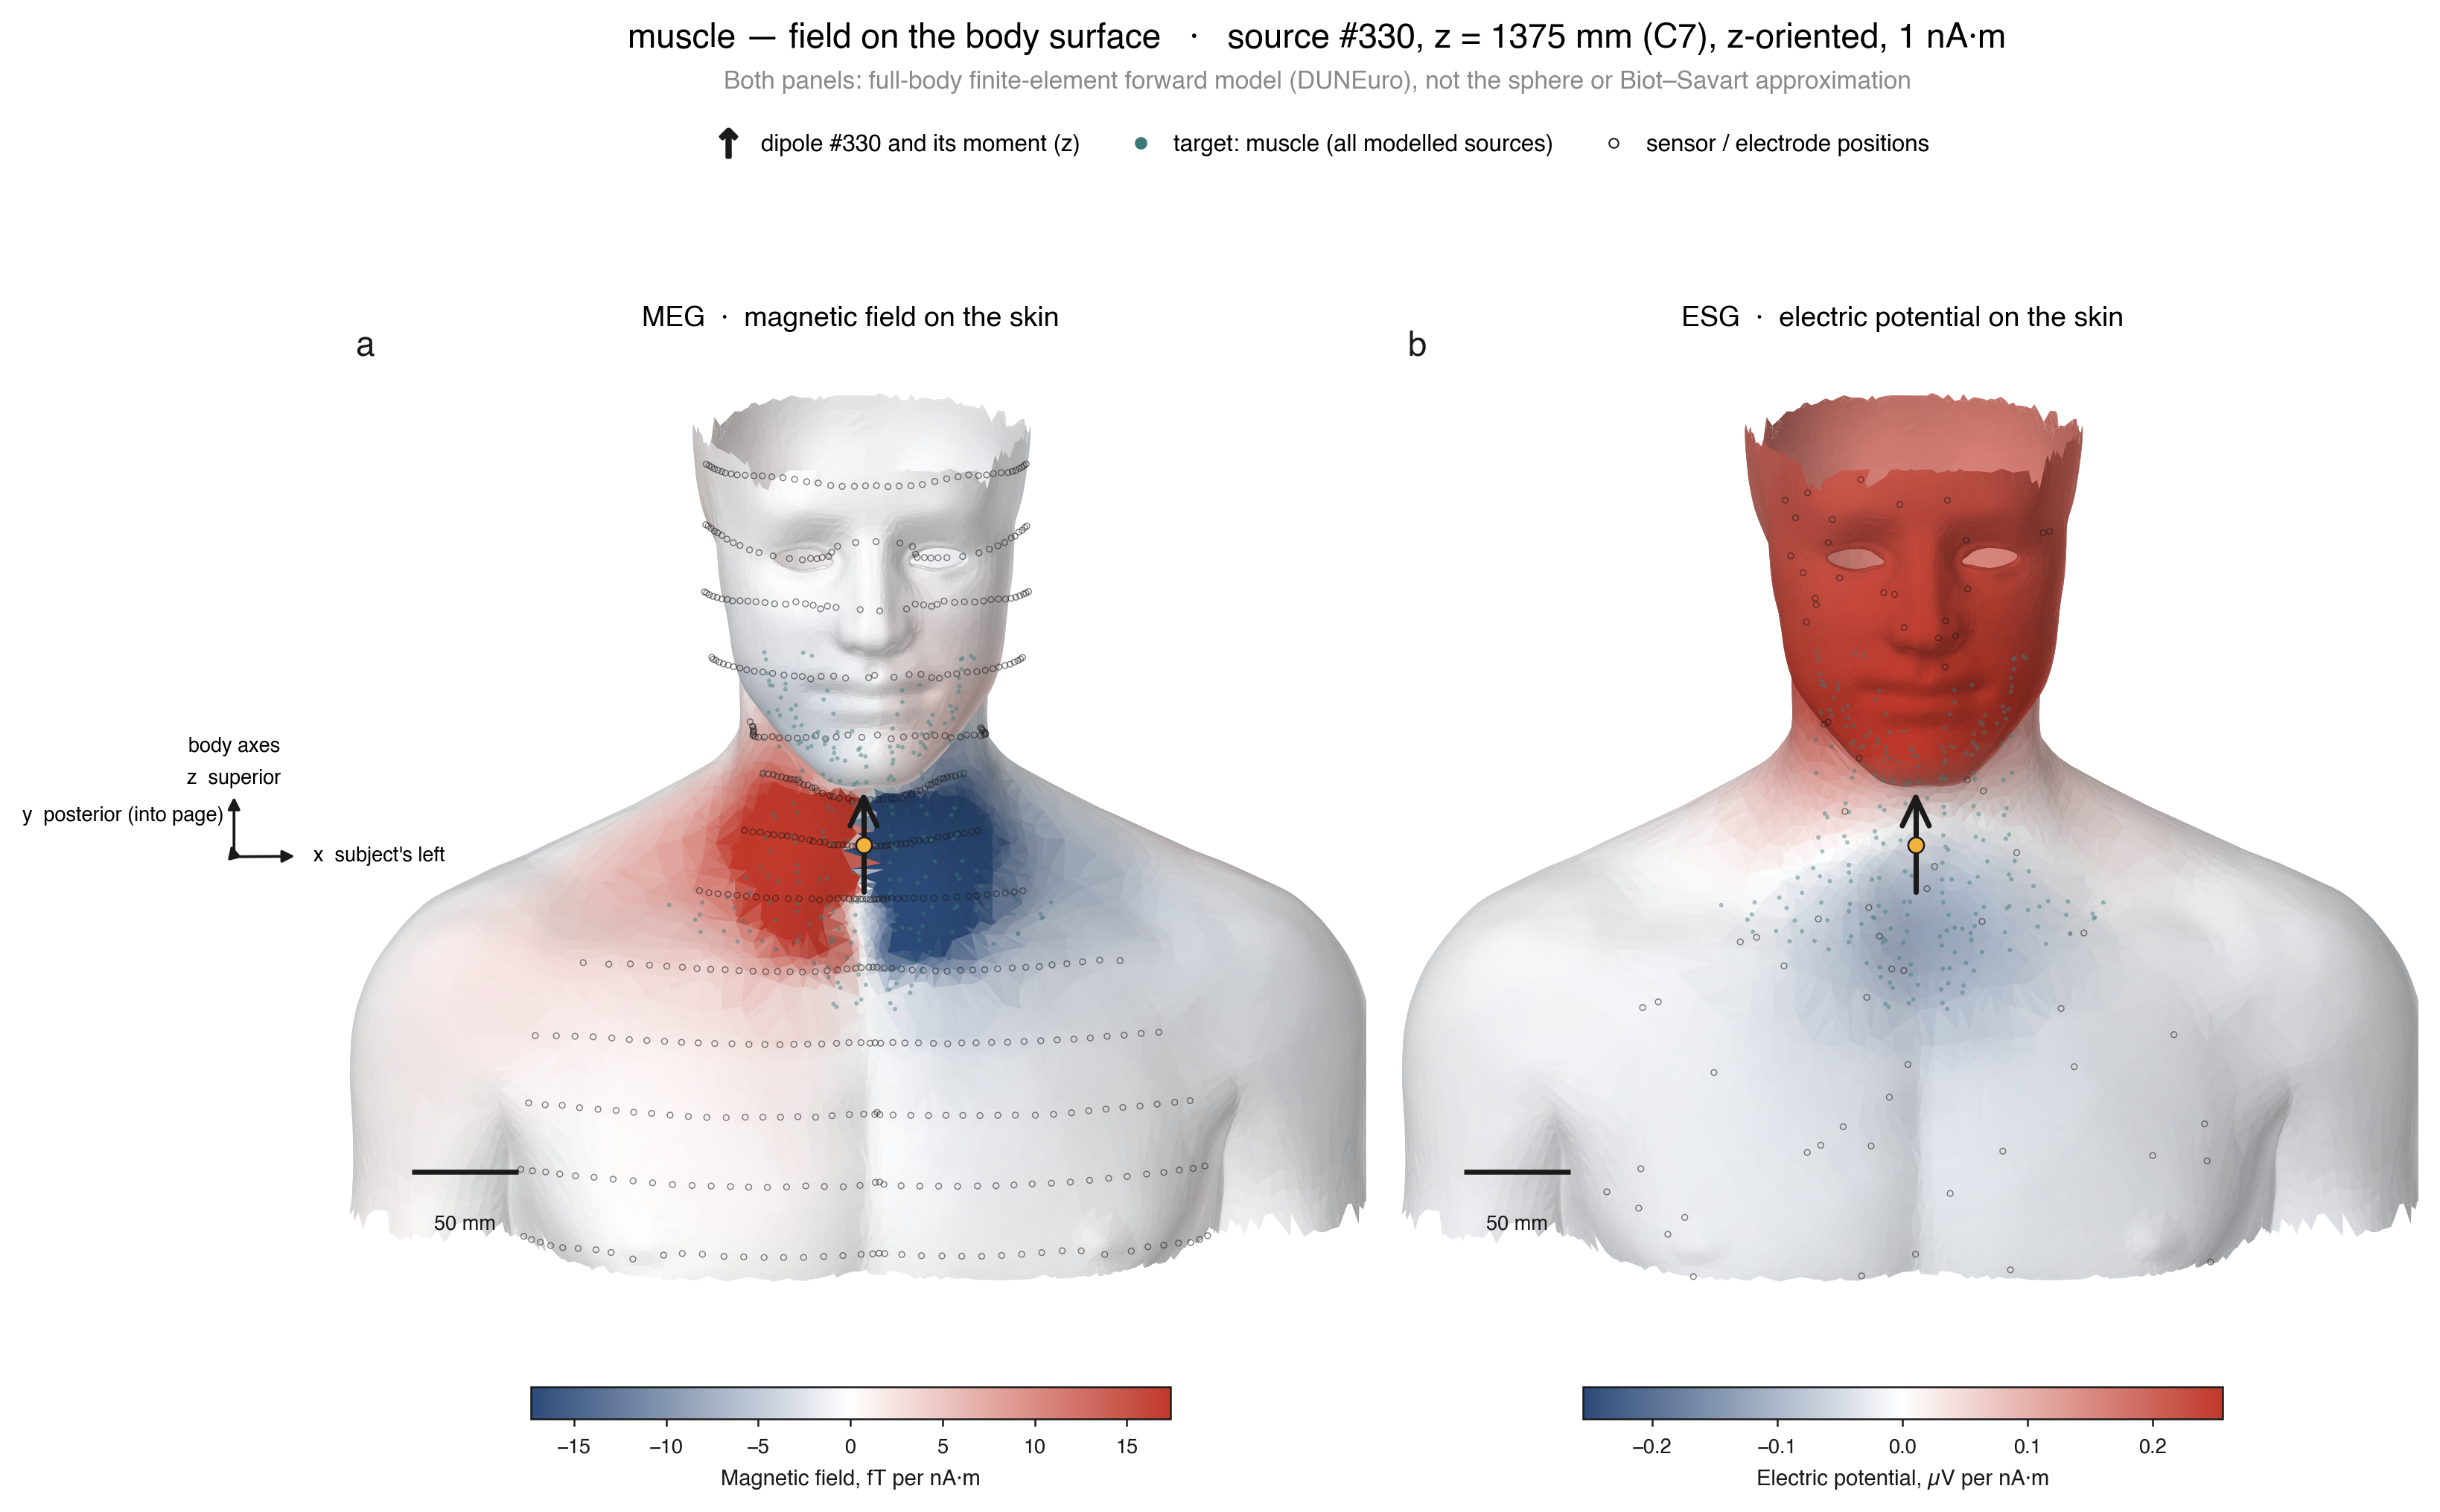
\includegraphics[width=\linewidth]{fig5_neck_muscles}
\caption{Neck muscle forward solution. Fields are shown for a
single z-oriented unit dipole (1 nA·m) in the \revised{anterior midline neck musculature} at \revised{z = 1375 mm, level C7 (source \#330 of 736),
drawn as an arrow along its moment in both panels; teal dots mark all
modelled muscle sources}. (a) Radial magnetic field on the skin, interpolated
from \revised{2,730 triaxial OPM positions at 30 mm pitch}; the dipolar pair sits
tight against the neck, \revised{two to three times stronger per unit moment than
the nerve sources} because the source is shallower\revised{, and splits
left from right about the midline}. (b) Surface electric potential
on the same skin\revised{, positive over the head and negative over the lower
neck and upper chest}, interpolated from \revised{1,000 whole-body electrodes
(\textasciitilde20 mm mean contact spacing)}, common-average referenced.
Both panels share mesh, camera, orthographic projection and scale (bar:
50 mm). Skin further than 1.6 × the array spacing from the nearest
sensor is left unpainted. Colour scales are symmetric about zero,
clipped to the 98th percentile of the measured surface \revised{(±17 fT per nA·m
in a; ±0.26 µV per nA·m in b)}, and are given beneath each panel.}
\label{fig:5}
\end{figure}

\section{Discussion}\label{discussion}

We present iNOB, an open-source package for whole-body
bioelectromagnetic forward modelling, able to treat any anatomical
region available in the underlying 3D mesh library. The package is not
an inverse-solution tool: individual geometry varies too much for a
single-atlas model to support source reconstruction in a given subject.
Its purpose is simulation for experimental design: it allows an
investigator to establish, before any data are collected, the type and
number of sensors required, where to place them, and how many averaged
trials would be required to detect a given source. It also indicates how
complex a forward model is needed, and therefore what individual
participant data (for example, anatomical imaging) should be collected.

\subsection{What the package is for}\label{what-the-package-is-for}

The intended use is experimental design. Before committing to a study,
an investigator can ask whether a given structure is reachable at all
with available sensors, how many trials would be required, where on the
body surface the array should be placed, and whether the electrical or
magnetic modality is better suited to the target. Our own examples
answer three such questions. For the cervical vagus, coupling varies
\revised{17-fold} along the nerve and trials-to-detect varies by two orders of
magnitude between its ends, so array placement is the most important
design decision, and electrode repositioning cannot rescue the
electrical measurement because the limiting factor is attenuation of the
surface potential across approximately 50 mm of conductive tissue rather
than coverage or bone. For the spinal cord, extending electrode coverage
over the whole body brings the trial count inside the clinical
somatosensory evoked potential range, but it also recruits progressively
larger muscle groups, so each added channel brings muscle artefact as
well as sensitivity. For muscle, detectability is never the question,
and the design problem is separability instead. The package can also
compare array placements directly\revised{: \texttt{inob placement -\/-optimise}
greedily chooses the positions that maximise the total information
carried about all sources in the target,
\(\tfrac{1}{2}\log_{2}\det(I + LCL^{\top}/\sigma^{2})\), the
channel-capacity measure of \citet{Schneiderman2014} as used for sensor
design by \citet{Iivanainen2021}, and writes the result as an array that
\texttt{inob sensors -\/-from} loads for a forward solve.} \revised{For a single
source, choosing sensors by predicted coupling rather than proximity
changes the matched-filter amplitude by 1--10\% (spine 0.99×, vagus
1.03×, muscle 1.10× at 20 sensors). Over a whole structure, the
information-optimised array carries 14--17\% more information than the
positions nearest the spinal cord for 4--16 sensors, falling to 1\% at
64; for muscle the difference is at most 1\%; and for the vagus the
greedy design does 5--6\% worse than the nearest positions, because
greedy selection under a minimum-spacing rule carries no optimality
guarantee.} \revised{This agrees with
\citet{Iivanainen2021}, who found that for large numbers of samples
uniform grids carry nearly the same total information as model-informed
ones, and extends that result to extracranial targets. For these
targets, proximity is therefore an adequate placement rule.}

The same machinery applies to targets we have not modelled. In future
work, we intend to extend iNOB to also model muscular and neural signals
from the heart, the stomach, the brachial plexus and the sympathetic
chain. Such an extension only requires a mesh, a conductivity assignment
and a source model, and magnetocardiography in particular offers an
abundant empirical literature against which the calibration could be
validated directly. We regard that validation as the highest-priority
extension. Supporting gradiometer arrays would require only that
leadfields computed at paired coil positions be differenced, which the
existing sensor definition could accommodate.

\subsection{Why model beyond the
brain}\label{why-model-beyond-the-brain}

The worked examples in Section 4 address individual targets, but the
case for a whole-body forward model is broader than any one of them.
Historically, cognition was thought to occur solely in the brain. It is
now recognised, however, that multiple bodily systems are involved in
how we process and understand the world around us. Interoceptive
signalling to the brain shapes central neural activity, informing, for
example, regulatory strategies and our sense of self \citep{44, 18}.
Interoceptive afferent signalling has been linked to memory \citep{229},
decision making \citep{230} and emotion \citep{231, 232}, and implicated
in the pathophysiology and treatment of different mental health
conditions (Nord \& Garfinkel, 2022). To fully understand neural
processing, we must therefore consider the body, and the autonomic and
peripheral nervous systems, in their entirety. Within the autonomic
nervous system, vagal afferent traffic, including baroreceptor
signalling, pulmonary stretch-receptor activity and cytokine-modulated
inflammatory-reflex signalling \citep{179}, is directly relevant to
cardiovascular risk and to post-viral syndromes causing dysautonomias
\citep{198}, as well as to interoception itself \citep{194, 197}.

Recording beyond the brain is not only relevant to interoception. These
signals can be measured, analysed and interpreted with the same
non-invasive tools already used for the head, and together they show
that we need to record from more than the brain alone. There is now a
growing appreciation that we, as a field, need to image beyond the brain
to understand cognition as a whole (Case, 2026, in review; Imaging
Neuroscience,\citep{225, 194}).

So far, the field has developed its strategies and deepened its
understanding of the nervous system almost entirely from information
about the brain. Yet much of our central nervous system, peripheral
nerves and the viscera sit outside our heads. By comparison with brain
imaging, minimal work has been done on electromagnetic recordings from
the rest of the nervous system. In part, this may be due to technology
and the rigidity historically imposed on experimental setups. We argue
here that to understand `the brain' as
a system, we must look below the skull. The body is critical to how we
perceive, interpret and react to our environment \citep{200, 201}, and
it, too, generates bioelectromagnetic signals that can add to our model
of neural processing \citep{199}. iNOB is intended to lower the barrier
to that step: by estimating, before any recording, whether a signal from
a given bodily structure is measurable and at what cost in trials, it
allows studies below the skull to be designed with the same rigour as
studies of the brain. Those estimates rest on a number of assumptions,
which we set out below.

\subsection{Limitations}\label{limitations}

The limitations of iNOB fall into three groups.

\textbf{Numerical.} The global voxel pitch is 3 mm by default; sub-voxel
structures are dilated by one voxel to survive rasterisation, so the
source compartment is partly a discretisation artefact. We have not yet
demonstrated convergence of the leadfield peak with decreasing voxel
pitch, and until we do, the absolute amplitudes should be treated as
accurate to within a factor that we cannot currently bound. \revised{Relatedly, the
electrography scale rests on dimensional analysis, confirmed on a
sphere by the median ratio to within 3\%; near shallow sources the 3 mm
mesh departs from the analytic potential by up to about 30\%, part of
the voxel-pitch convergence that has not yet been shown.}

\textbf{Anatomical and physical.} Conductivities are isotropic except
for muscle, frequency-independent, and taken as point values from the
IT'IS database rather than propagated as distributions;
the muscle anisotropy tensor is applied only where muscle is itself a
source, so in the vagus and cord runs the surrounding musculature, which
carries much of the return current, is treated as isotropic. The anatomy
derives from a single adult male atlas, so sex differences and
individual variation in tissue geometry, nerve course and body habitus
are not represented. The quasi-static approximation is assumed throughout
without being tested at the upper end of the compound action potential
spectrum.

\textbf{Detection model.} Noise is modelled as spatially white within a
30--500 Hz band. Correlated environmental interference would inflate
trials-to-detect and spatial filtering would reduce it; neither is
modelled, so the reported figures carry an uncertainty that we have not
resolved. Both floors are also instrument-only. As a check, we solved
brain MG and EG leadfields on the same whole-body FEM with the same
noise floors: the leadfield magnitudes are as expected for the brain
(for a 10 nA·m dipole 0--20 mm below the scalp, \revised{≈2.5 pT} at an on-scalp
OPM and \revised{≈5.3 µV} at the scalp), but the EG SNR is only \revised{0.20--0.45} times
the MG SNR across source depths of 0--60 mm, whereas, empirically, evoked
MEG and EEG SNRs are broadly comparable (Goldenholz et al., 2009). This
points to the noise model rather than the forward model as the source of
the large MG advantage reported in the worked examples, and the
MG-versus-EG comparisons should be read as holding under
instrument-limited noise only. The Rose criterion of SNR 3 is inherited
from imaging and is not a detection-theoretic statement about a time
series. The source model treats compound action potentials as biphasic
Gaussians with no fibre-diameter dispersion beyond the conduction
velocity assignment, no recruitment or firing-rate model for muscle, and
no postsynaptic component, which matters for the spinal cord because a
real somatosensory evoked response carries a dorsal horn contribution
that does not travel. The muscle case models only the motor unit action
potential, an evoked-stimulation analogue; the broadband isometric
contraction by which the neck musculature stabilises the head is not
represented.

None of these is fundamental to the design. Voxel pitch, conductivity
distributions, anisotropy assignment and noise model are all
configuration choices in the existing package rather than architectural
constraints, and the natural next steps are a convergence study, Monte
Carlo propagation of conductivity uncertainty, subject-specific meshes
(users can already point each tissue in the configuration at their own
surface meshes, for example from automated whole-body segmentation or
segmented MRI, within the fixed tissue set), and validation against
magnetocardiographic recordings where ground truth is plentiful.

\subsection{Conclusion}\label{conclusion}

The tools that allow source imaging of electrophysiology in the brain
are not, in principle, restricted to the brain; indeed, biomagnetic
measurement of the heart preceded that of the brain. What has restricted
them is that most components of the standard forward pipeline assume a
head. iNOB removes that assumption and, for the first time in a single
open package, allows an investigator to specify any structure included
in the atlas and obtain a calibrated estimate of what a sensor on the
skin would measure and what it would cost to measure it. The estimates
it currently produces are physical upper bounds (necessary rather than
sufficient conditions for detection) rather than estimates of what will
be achieved in practice, and moving closer to realistic and
individualised simulations is the next task. An upper bound, however, is
enough to answer the question that matters at the design stage: whether
an experiment is worth attempting at all. The key next step is an
empirical test of whether recordings match these simulations.

\section{Data and code availability}\label{data-and-code-availability}

\revised{The figure scripts are available on GitHub}. \revised{Solved leadfields are not distributed;
every leadfield, figure and number in this paper is regenerated from the
repository by \texttt{scripts/run\_all\_targets.sh} and
\texttt{scripts/paper\_numbers.py}, as described in
\texttt{docs/REPRODUCE.md}.}
Raw BodyParts3D meshes are available from the DBCLS Anatomography portal
under CC BY-SA 2.1 Japan. The full iNOB package is released under the
MIT licence; DUNEuro is available under the LGPL, with local and cluster
build scripts provided. Archived, citable releases are listed below.

\begin{center}
\small
\renewcommand{\arraystretch}{1.35}
\begin{tabular}{@{}>{\raggedright\arraybackslash}p{0.43\linewidth}l>{\raggedright\arraybackslash}p{0.33\linewidth}@{}}
\toprule
\textbf{Resource} & \textbf{Archive} & \textbf{Identifier} \\
\midrule
iNOB software package, v1.1.0~\citep{case2026inobzenodo} & Zenodo & \doilink{10.5281/zenodo.22688957} \\
iNOB project record~\citep{case2026inobosf} & OSF & \doilink{10.17605/OSF.IO/U4MDS} \\
BodyParts3D 4.3 verified mesh set, downloader and subset selector~\citep{case2026bodyparts} & Zenodo & \doilink{10.5281/zenodo.22727172} \\
\midrule
iNOB source code & GitHub & \href{https://github.com/olivercase/iNOB}{\nolinkurl{github.com/olivercase/iNOB}} \\
Curated BodyParts3D mesh inputs & GitHub & \href{https://github.com/olivercase/body_parts_3d_api}{\nolinkurl{github.com/olivercase/body_parts_3d_api}} \\
DUNEuro build scripts & GitHub & \href{https://github.com/olivercase/duneuro-build}{\nolinkurl{github.com/olivercase/duneuro-build}} \\
\bottomrule
\end{tabular}
\end{center}

\section{Funding}\label{funding}

\begin{center}
\small
\renewcommand{\arraystretch}{1.35}
\begin{tabular}{@{}>{\raggedright\arraybackslash}p{0.40\linewidth}>{\raggedright\arraybackslash}p{0.26\linewidth}>{\raggedright\arraybackslash}p{0.26\linewidth}@{}}
\toprule
\textbf{Funder} & \textbf{Grant} & \textbf{Recipient} \\
\midrule
British Heart Foundation (BHF) & SI/F/24/21170016 & This research \\
British Heart Foundation (BHF) & RG/F/25/110148 & This research \\
Wellcome, Discovery Research Platform for Naturalistic Neuroimaging & 226793/Z/22/Z & This research \\
Wellcome Mental Health Award & 226778/Z/22/Z & S.N.G. \\
\bottomrule
\end{tabular}
\end{center}

The funders had no role in study design, analysis, the decision to
publish or preparation of the manuscript.

\section{Conflict of interest}\label{conflict-of-interest}

The authors declare that the research was conducted in the absence of
any commercial or financial relationships that could be construed as a
potential conflict of interest.

\section{Ethics statement}\label{ethics-statement}

No new human or animal data were collected. All anatomical content
derives from the open BodyParts3D atlas; therefore, ethical approval was
not required.

\section{CRediT author statement}\label{credit-author-statement}

\textbf{Oliver Case:} Conceptualisation, Methodology, Software,
Validation, Formal analysis, Investigation, Data curation, Writing --
original draft, Writing -- review \& editing, Visualisation, Project
administration. \textbf{Maike Schmidt:} Conceptualisation, Methodology,
Software, Validation, Formal analysis, Investigation, Writing -- original
draft, Writing -- review \& editing, Visualisation. \textbf{Harry Cook:}
Software, Validation, Investigation, Writing -- review \&
editing. \textbf{Pier D. Lambiase:} Supervision, Funding acquisition,
Writing -- review \& editing. \textbf{Sarah N. Garfinkel:} Supervision,
Funding acquisition, Resources, Writing -- review \& editing.
\textbf{Gareth R. Barnes:} Conceptualisation, Supervision, Funding
acquisition, Resources, Writing -- review \& editing.

\bibliographystyle{plainnat}
\bibliography{references}

\end{document}
